\chapter{$sp^3$ defect in Biased Bilayer Graphene}
\label{ch:vacancy_bilayer}
%\section{Introduction [not serious]}
%Theoretical Physicist have been dreaming with theoretical models since they realized it was much easier to write down and solve some equations than find a material governed by such equations. For years without end, we have created more and more models, useful, and boring, and silly, and interesting ones, but just theoretical models non the less.
%
%The problem of vacancies/adatoms in graphene has been widely studied, both theoretically and experimentally. On one hand, the experimental studies usually focus on the local properties of the localized states, lacking the capability to study ``complex'' structures of vacancies/adatoms. On the other hand, theoretical studies usually relay on calculations in which the translational symmetry of the crystal is preserved, what is generally considered a handicap for the model since experimentally the vacancies do not form an array large enough to behave as a crystal. Any effect derived from the consideration of a crystal of vacancies is usually neglected either as an artifact of the theory or an unachivable experimental option. If this limitation is avoided, then the theoretical study focus in single vacancies as experimental studies usually do.
%
%Recent experimental advances have shown the capability to arrange large areas/quantities of atoms with atomic precision\cite{Brihuega2016,Kalff2016}.
%An obvious question is whether or not we can build artificial lattices by placing adatoms on graphene.
%
%The idea is to use a large flake of graphene bilayer (the reasons will be explored later in the text) in which the adatoms are placed in very specific atomic positions to form a (periodic) crystal. Since graphene can be described with a triangular or a rectangular Bravais lattice, many crystals are available by choosing the suitable unit cell and lattice vectors.
%
%
%There are two main reasons to choose graphene bilayer as the platform to build artificial fermion models. The first one is that graphene (and by extension graphene bilayer) is the most studied material ever. The fabrication and tuning capabilities exceeds those of any other material. The second one is that its electronic properties are highly tunable whether it is via proximity to other materials or via the application of external fields.

% XXX move
% When an external electric field is applied to graphene bilayer, a tunable gap is open\cite{Zhang2009,Lui2011,Ponomarenko2011} (the maximum observed value is $\Delta_E\sim\SI{0.25}{\eV}$).


%\section{General considerations} %~~~~~~~~~~~~~~~~~~~~~~~~~~~~~~~~~~~~~~~~~~~~~%
%We are going to study the electronic states arose by vacancies in the $\pi$-manifold in graphene bilayer (GB) and its interactions with an external electric field, $V$.
%We will consider isolated vacancies in order to study the properties of the electronic states. Later on, we will also study infinite periodic arrays of defects forming a crystal.\\
%
%When only a finite number of vacancies are considered, the system used will be an armchair island, as such, the system is $0$-D, so there is no translational symmetry and no $\vec{k}$ vector can be defined, nor Bloch's theorem can be applied.
%
%To study these systems we will consider a basis of localized states that could be considered to be the $p_z$ hydrogenoid orbitals.
%\begin{equation}
%  \mathcal{B} = \left\{\phi_1,\phi_2,\dots,\phi_\alpha,\dots,\phi_{N_C}\right\}
%\end{equation}
%
%The complete Hamiltonian will look like this:
%\begin{equation}
%  H = H_t + H_{t'} + H_{V}
%\label{hamiltonian}
%\end{equation}
%
%The term $H_t$ represents the kinetic energy arising from the hopping between neighboring sites in the same layer, $H_{t'}$ represents the interlayer hoppings and the term $H_{V}$ corresponds to the effect of an external electric field on the electrons. Such a term is considered to be just a layer dependent shift in the on-site energies:
%% \begin{equation}
%%   H_{\lambda_E} = \lambda_E
%%   \left(\begin{array}{cc}
%%   \mathds{1} & 0 \\
%%   0 & -\mathds{1}
%%   \end{array}\right)
%% \end{equation}
%\begin{equation}
%  H_{V} = V\lambda_l
%\end{equation}
%where $V$ is the potential difference between the two layers and $\lambda_l\in\{-1,1\}$ labels the layer.
%The vacancies are introduced in this model as an infinite on-site energy for the chosen atom(s). Unless otherwise stated, everything is done in $eV$, \emph{not in hopping units}. The intralayer $p_z$-$p_z$ hopping is chosen as $t=\SI{-2.7}{\eV}$ and the interlayer $t'=\SI{0.4}{\eV}$ in accordance with the literature\cite{KatsnelsonBook}.\\
%
%In the presence of vacancies, there will appear in-gap states (as many as vacancies are considered) which will be labeled by $\Psi_0$, $\Psi_1$, ... in order to distinguish them form any other eigenstate.
%\begin{equation}
%\begin{split}
%  H\ket{\psi_\alpha} = E_\alpha\ket{\psi_\alpha} \qquad&;\qquad
%\ket{\psi_\alpha} = \sum_\beta c_\beta\ket{\phi_\beta}\\
%  H\ket{\Psi_0} &= E_0\ket{\Psi_0}
%\end{split}
%\end{equation}
%
%%  \section{Effects of an external electric field}
%%  
%%  In order to open a gap in the band structure of graphene bilayer one has to apply an external electric field. One option would be to simply place an electric gate under the sample, but this approach will heavily charge the system as soon as free charges are available (for instance from a hypothetical source and drain contacts)\cite{McCann2006,Zhang2009,Taychatanapat2010}.
%%  The other option is to use two gates, one on top of the sample and the other underneath it. Let us discuss the second option.
%%  
%%  
%%  \subsection{Dual Gating}
%%  Let us consider a graphene bilayer, depicted by the black lines and balls in Fig.~\ref{dual_gate}, sandwiched by $SiO_2$ layers and with two gates, unoriginally referred to as top and bottom, each with a voltage $V_{t/b}$ respectively. This setup will be consider as an infinite parallel plate capacitor.
%%  %~~~~~~~~~~~~~~~~~~~~~~~~~~ FIGURE ~~~~~~~~~~~~~~~~~~~~~~~~~%
%%  \begin{figure}[h!]
%%  \centering
%%  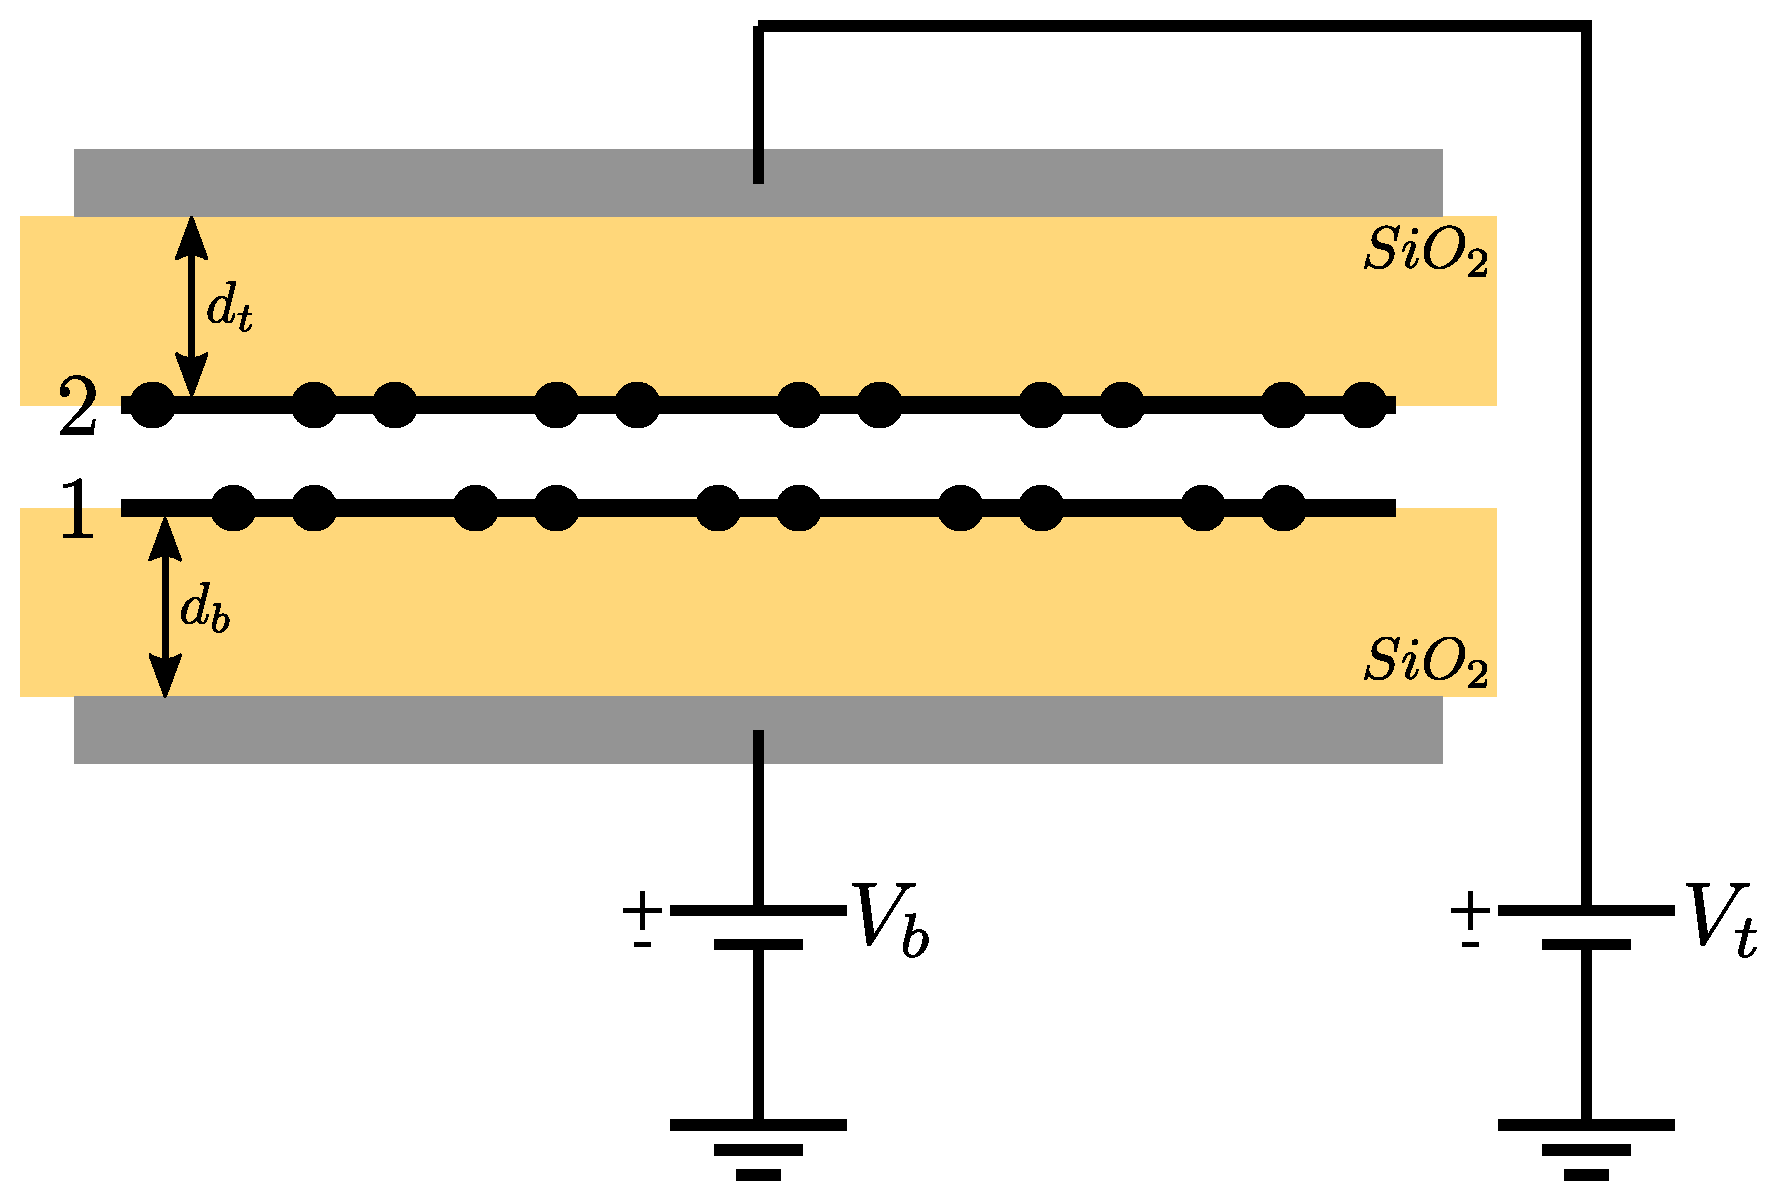
\includegraphics[width=0.5\textwidth]{artlat/fig/dual_gate.pdf}
%%  \vspace{-5pt}
%%  \caption{Schematics of dual gating.}
%%  \label{dual_gate}
%%  \end{figure}
%%  \FloatBarrier
%%  %~~~~~~~~~~~~~~~~~~~~~~~~~~~~~~~~~~~~~~~~~~~~~~~~~~~~~~~~~~~%
%%  
%%  The role of the electric field induced by the voltage $V_t$ and $V_b$ is twofold. On one hand, it will break the symmetry between the two layers by shifting their on-site energies, on the other hand it may dope the  system.
%%  
%%  The doping (extra charge absorbed into the system) in the graphene bilayer can be estimated simply by applying Gauss' law:
%%  \begin{equation}
%%     \diver{D} = \rho-\rho_0 = \rho_f
%%  \label{gauss}
%%  \end{equation}
%%  where $\rho$ is total charge density, $\rho_0$ is the bounded charge density so that $\rho_f$ is the free charge density.
%%  
%%  Since we are considering an infinite capacitor, the electric field only has $z$ component, hence the divergence of the displacement results in a derivative which can be discretized:
%%  \begin{equation}
%%     \diver{D}=\frac{\partial D}{\partial z} =\frac{D_t-D_b}{dz} = \rho_f =
%%     e\frac{N}{V} \Rightarrow D_t-D_b = e\delta n
%%  \label{doping}
%%  \end{equation}
%%  where $N$ and $V=Adz$ are the number of electrons and volume ($A$ is the area), and $\delta n$ is the bidimensional density of electrons.
%%  
%%  In order to calculate the potential difference between the two graphene layers, we can consider simply the average of the electric field inside the capacitor:
%%  \begin{equation}
%%     \Delta V = \langle\vec{E}\rangle \Delta z = \frac{E_t+E_b}{2} \Delta z=
%%     \frac{\Delta z}{2} \left(\frac{D_t}{\varepsilon_t} +
%%                              \frac{D_b}{\varepsilon_b} \right)
%%  \label{potential}
%%  \end{equation}
%%  where $\Delta z$ is width of the graphene bilayer and $\varepsilon_t$ and $\varepsilon_b$ are the electric permeability of the top and bottom dielectrics. $D_t$ and $D_b$ are (the $z$-component of) the displacement fields in the top and bottom regions.
%%  \begin{equation}
%%     D_t = \frac{\varepsilon_t}{d_t}\left(V_{t}-V^0_{t}\right) \qquad;\qquad
%%     D_b = \frac{\varepsilon_b}{d_b}\left(V_{b}-V^0_{b}\right)
%%  \end{equation}
%%  where $V^0_{t/b}$ are the off-set potential required to have charge neutrality, usually referred to as \ac{cnp}.
%%  
%%  Equations \eqref{doping} and \eqref{potential} show that by choosing the appropriates $V_t$ and $V_b$ we can independently change the doping of the system and the gap opened in the band structure.
%%  
%%  
%%  
%%  \subsection{Hartree}
%%  Using the basis $\mathcal{B}=\left\{\phi^1_A,\phi^1_B,\phi^2_A,                 \phi^2_B\right\}$ (where $A/B$ label sublattice and $1/2$ label the graphene    layer) we can write the basic Hamiltonian that models a graphene bilayer as:
%%  \begin{equation}
%%     H(\vec{k}) = \left(\begin{array}{cccc}
%%           \epsilon_1 & f(\vec{k}) & 0 & 0 \\
%%           f^*(\vec{k}) & \epsilon_1 & \gamma & 0 \\
%%           0 & \gamma & \epsilon_2 & f(\vec{k}) \\
%%           0 & 0 & f^*(\vec{k}) & \epsilon_2
%%                  \end{array}\right)
%%  \end{equation}
%%  where $\epsilon_{1/2}$ account for both the shifting of the on-site energies  in each layer and the effect of having extra charge in the opposite layer.
%%  \begin{equation}
%%  \begin{split}
%%     \epsilon_1 &= \frac{e}{\varepsilon_0}\Delta z \sigma_2 + V^0_1 \\
%%     \epsilon_2 &= \frac{e}{\varepsilon_0}\Delta z \sigma_1 + V^0_2
%%  \end{split}
%%  \end{equation}
%%  where $\sigma$ is the planar charge density, calculated as:
%%  \begin{equation}
%%     \sigma_{\text{bottom}} = \sum^{N_{\text{occ}}}_i |\bra{\psi_i}\mathcal{O}_B \ket{\psi_i}|^2
%%     \frac{e}{N_k A}
%%  \end{equation}
%%  Each of the Hartree contributions, then will be:
%%  \begin{equation}
%%     \epsilon^{H}_1 = \frac{e^2\Delta z}{\varepsilon_0A}
%%     \frac{1}{N_k}\sum|\mean{B}|^2
%%  \end{equation}
%%  The order of magnitude of the prefactor is:
%%  \begin{equation}
%%     \frac{e^2\Delta z}{\varepsilon_0A} =
%%     \frac{\SI{2.56e-38}{\coulomb\squared} \cdot \SI{3.1e-10}{\meter}}
%%     {\SI{8.8e-12}{\coulomb\per\volt\per\meter} \cdot \SI{5e-20}{\meter\squared}}=
%%     \SI{1.75e-17}{\joule} \sim \SI{109.23}{\eV}
%%  \end{equation}
%%  where we have used that $\si{\joule}=\si{\coulomb\volt}$. The remaining factor $\tfrac{1}{Nk}\sum\langle B\rangle\sim 0.5$ since $|\mean{B}|^2\in[0,1]$
%%  
%%  
%%  
%%  The calculation of the first terms, has to be done iteratively since the estimation of electronic density, $\delta n$, depends on the eigenfunctions of the system, which depends on the on-site energies which depend on the electronic density.
%%  
%%  %
%%  % XXX Calculate and describe the Hartree solution
%%  %
%%  
%%  





%\section{Biased bilayer graphene}
%The electronic structure of bilayer graphene in the presence of an external electric field has been widely studied. Here I summarize the basic relevant properties.\\
%%~~~~~~~~~~~~~~~~~~~~~~~~~~ FIGURE ~~~~~~~~~~~~~~~~~~~~~~~~~%
%\begin{figure}[!ht!]
%\centering
%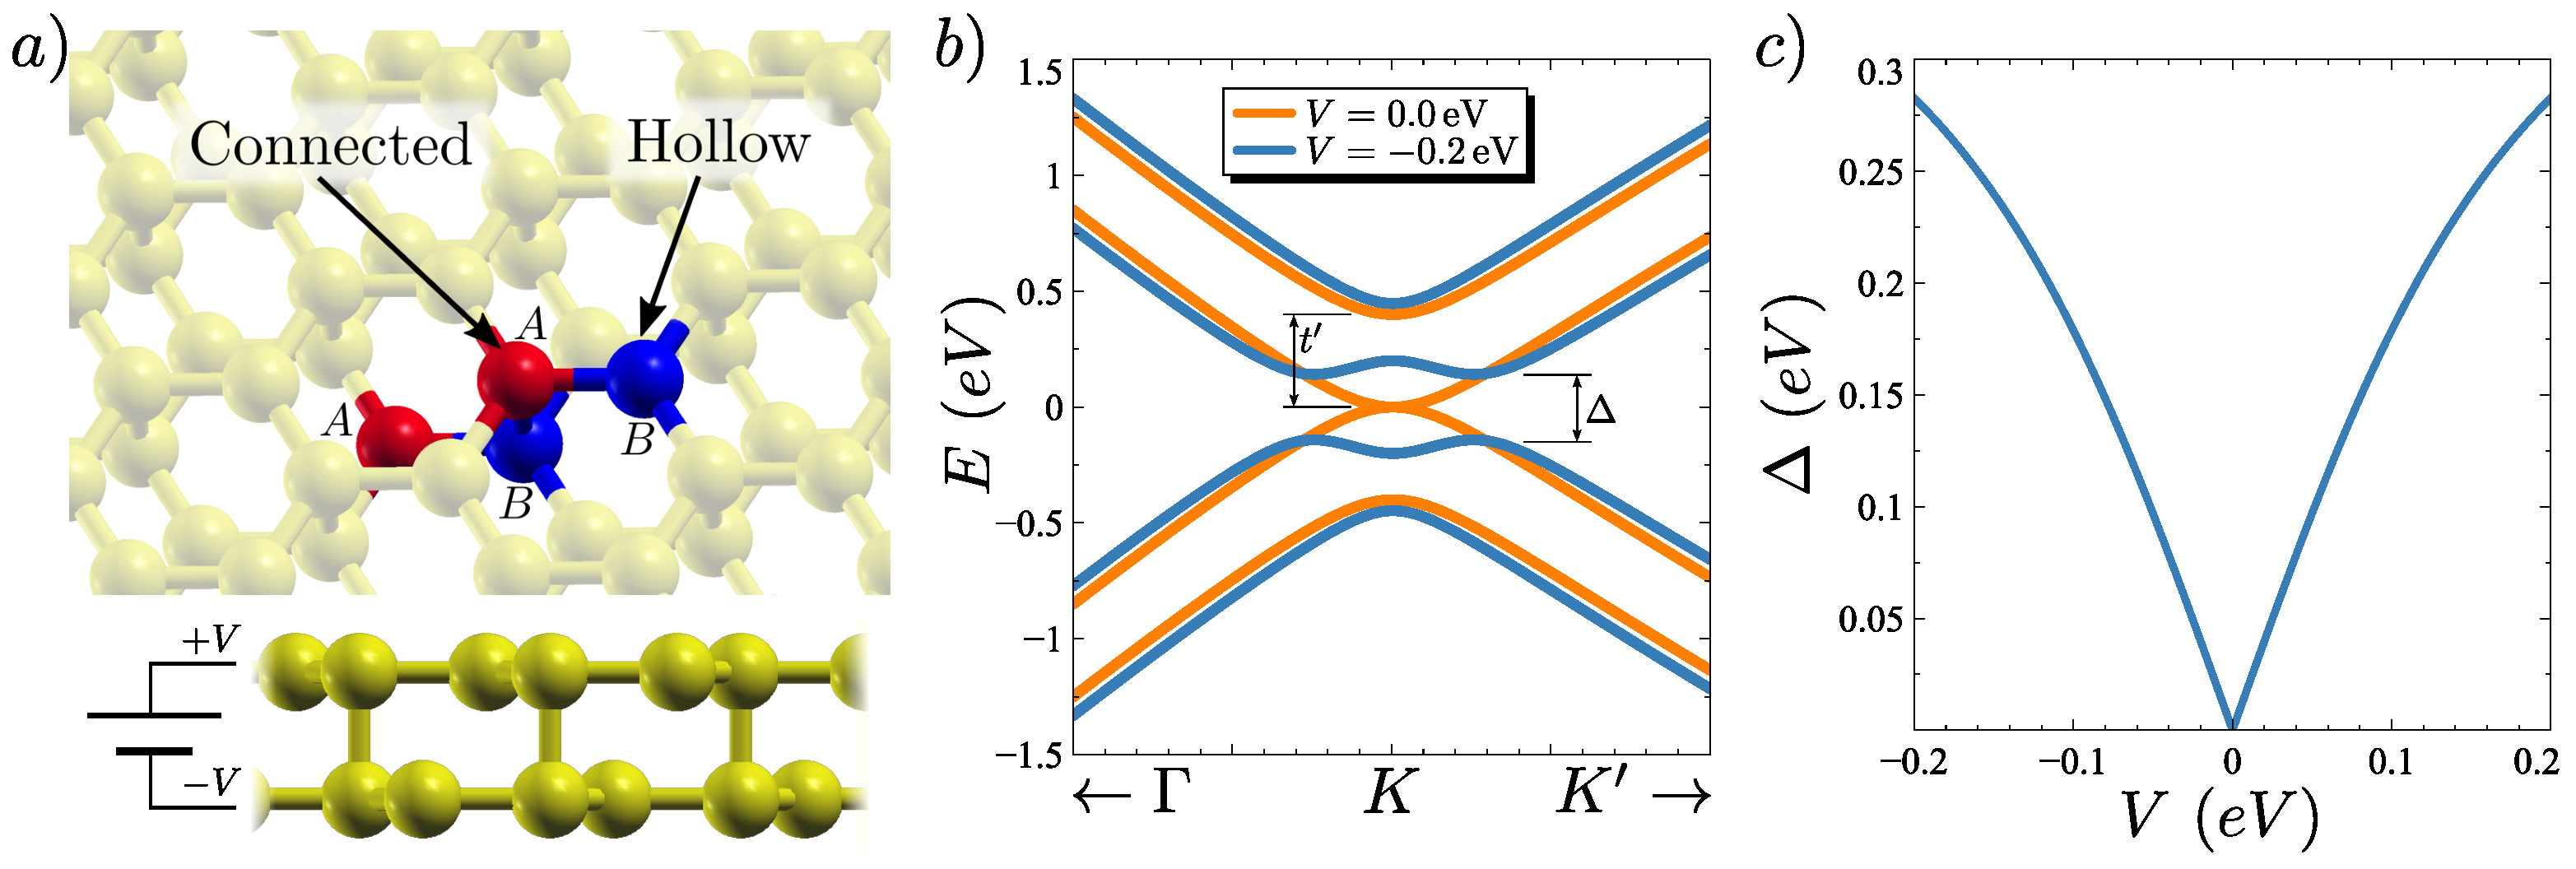
\includegraphics[width=0.9\textwidth]{artlat/fig/bands_bilayer.pdf}
%\vspace{-5pt}
%\caption{$a)$ Sketch of the minimal unit cell for graphene bilayer and disposition of the external electric field. Notice the two possibilities for placing the vacancies, we will focus on the hollow sites. $b)$ band structure of graphene bilayer with (blue) and without (orange) electric field. $c)$ Dependence of the gap open by the electric field. Notice that the gap is no longer at $K$, as shown in panel $b)$.}
%\label{bilayer2d}
%\end{figure}
%% \FloatBarrier
%%~~~~~~~~~~~~~~~~~~~~~~~~~~~~~~~~~~~~~~~~~~~~~~~~~~~~~~~~~~~%
%Rather than having a linear band structure, bilayer graphene presents parabolic bands around the $K$ point. It has zero gap, and the next bands are split by the interlayer hopping $t'$. When an external electric field is switched on, a gap is open at the $K$ point as shown in Fig.~\ref{bilayer2d} $b)$ and $c)$. The band gap behaves linearly for small electric fields while it tends to saturation when the gap is comparable to the interlayer splitting governed by $t'$.
%
%This calculation is not exactly accurate with the experimental results\cite{Zhang2009} since it does not consider any self-consistent or screening effect at all, nevertheless it contains the necessary ingredients to describe the relevant physics of the problem, so for the sake of simplicity we will remain at this level of description.

In the previous chapters we have covered the basic properties of monolayer and bilayer graphene as well as the effects of single $sp^3$ defects on monolayer graphene. The simplest case, deposition of \ce{H} adatoms, which can also be described as vacancies in the $p_z$ lattice, result in a quasi-localized electronic state with a certain magnetic moment. In this chapter we expand the study to bilayer graphene. Naturally many of the results will be similar, but bilayer graphene introduces a crucial property: An electrically controlled gap opening.


Pristine, infinite, bilayer graphene does not present a band gap. Unlike monolayer graphene, bilayer graphene does have a finite (although tiny) density of states at $E=0$. Its states around the Fermi energy are completely delocalized among the $p_z$-manifold of the two graphene layers it is made of.

An external perpendicular electric field can turn the usual conducting bilayer graphene into an insulator by opening a band gap as big as\cite{McCann2006, Castro2007, Oostinga2007, Zhang2009, Taychatanapat2010, Castro2010a, Ponomarenko2011, Allen2012, Sui2015} $\Delta\sim\SI{250}{\meV}$.
It is no surprise that such a phenomena has a huge impact on the low energy states around the Fermi energy. In particular, it crucially affects the localization and extension of these states.

The electrically controllable band gap, in addition to the capability of the $sp^3$-defects to quasi-localize electrons will be the cornerstone of our proposal for several applications for biased bilayer graphene.
\medskip


% In the previous chapter we studied the effect of a single $sp^3$ defect in graphene which main effect was the appearance of a resonant state at the Fermi Energy, mainly localized around the defect but extended all over the system.
% \smallskip

The results for the monolayer are a good reference for what might happen in bilayer graphene. Indeed the presence of $sp^3$-defects quasi-localizes electrons around them, but their properties depend strongly on where the defect is placed. This dependence is due to the asymmetric role of each sublattice in each of the layers.


\section{The finite system}
Just like in the previous chapter, the introduction of a defect breaks the translational symmetry, so no Bloch description is possible and there is no band structure to talk about. In the previous chapter we used the embedding technique to circumvent the issue but this method is only good enough for getting the Green's function. It is not able to retain the wave-function information, which will be necessary later on.
Instead, we will use a finite system which, for a big enough number of atoms should capture the relevant behavior of the infinite system it mimics.
\medskip


In order to retain the wave function information we are going to consider a huge but finite hexagonal island with armchair edges. We chose the island to have armchair edges so we can avoid the edge states at the Dirac point present in systems with zig-zag edges.\cite{Nakada1996}
%We will consider a big enough island so we can neglect the edge effects.
We will discuss the effects of the size on the properties and take care that any conclusion is appropriately converged so we are not misled by calculation artifacts. The largest island will be $\sim\SI{50.6}{\nm}$ in diameter, containing 131772 atoms\footnote{This limit is based solely upon RAM and patience, it would be feasible to keep increasing it.}.  % limit RAM-patience


We will calculate the spectrum of the system, comparing the pristine and defected cases and explore the properties of its wave functions. Of course, the brute force full diagonalization of a $131772\times131772$ Hamiltonian is, at the very least, challenging for any standard computer, so we will use Lanczos diagonalization\cite{Lanczos1950, Ojalvo1970, Arnoldi1951} to obtain only the 9 eigenvalues closest to the Fermi energy\footnote{The number of eigenvalues to obtain is arbitrary although Lanczos diagonalization is better suited, and efficient, for a small number of them.}.

Since the spectrum will usually be calculated for different electric fields, $\mathcal{E}$, each spectrum will be plotted next to each other in order to see the smooth evolution of the system with the electric field. This way of displaying the properties is very useful but it may fool the eye since the final result resembles somehow a band structure (see \fref{fig:hollow-connected}b) and e), for instance) but it is important to keep in mind that, unless stated, we will be dealing with finite systems, so we can only obtain discrete spectra.


\section{Hollow vs. Connected sites}
There are two inequivalent places where an adatom can be deposited in AB-stacked bilayer graphene, shown in \fref{fig:hollow-connected}a) and d). They are inequivalent due to the different role each sublattice plays.

%~~~~~~~~~~~~~~~~~~~~~~~~~~ FIGURE ~~~~~~~~~~~~~~~~~~~~~~~~~%
\begin{figure}[h!]
\centering
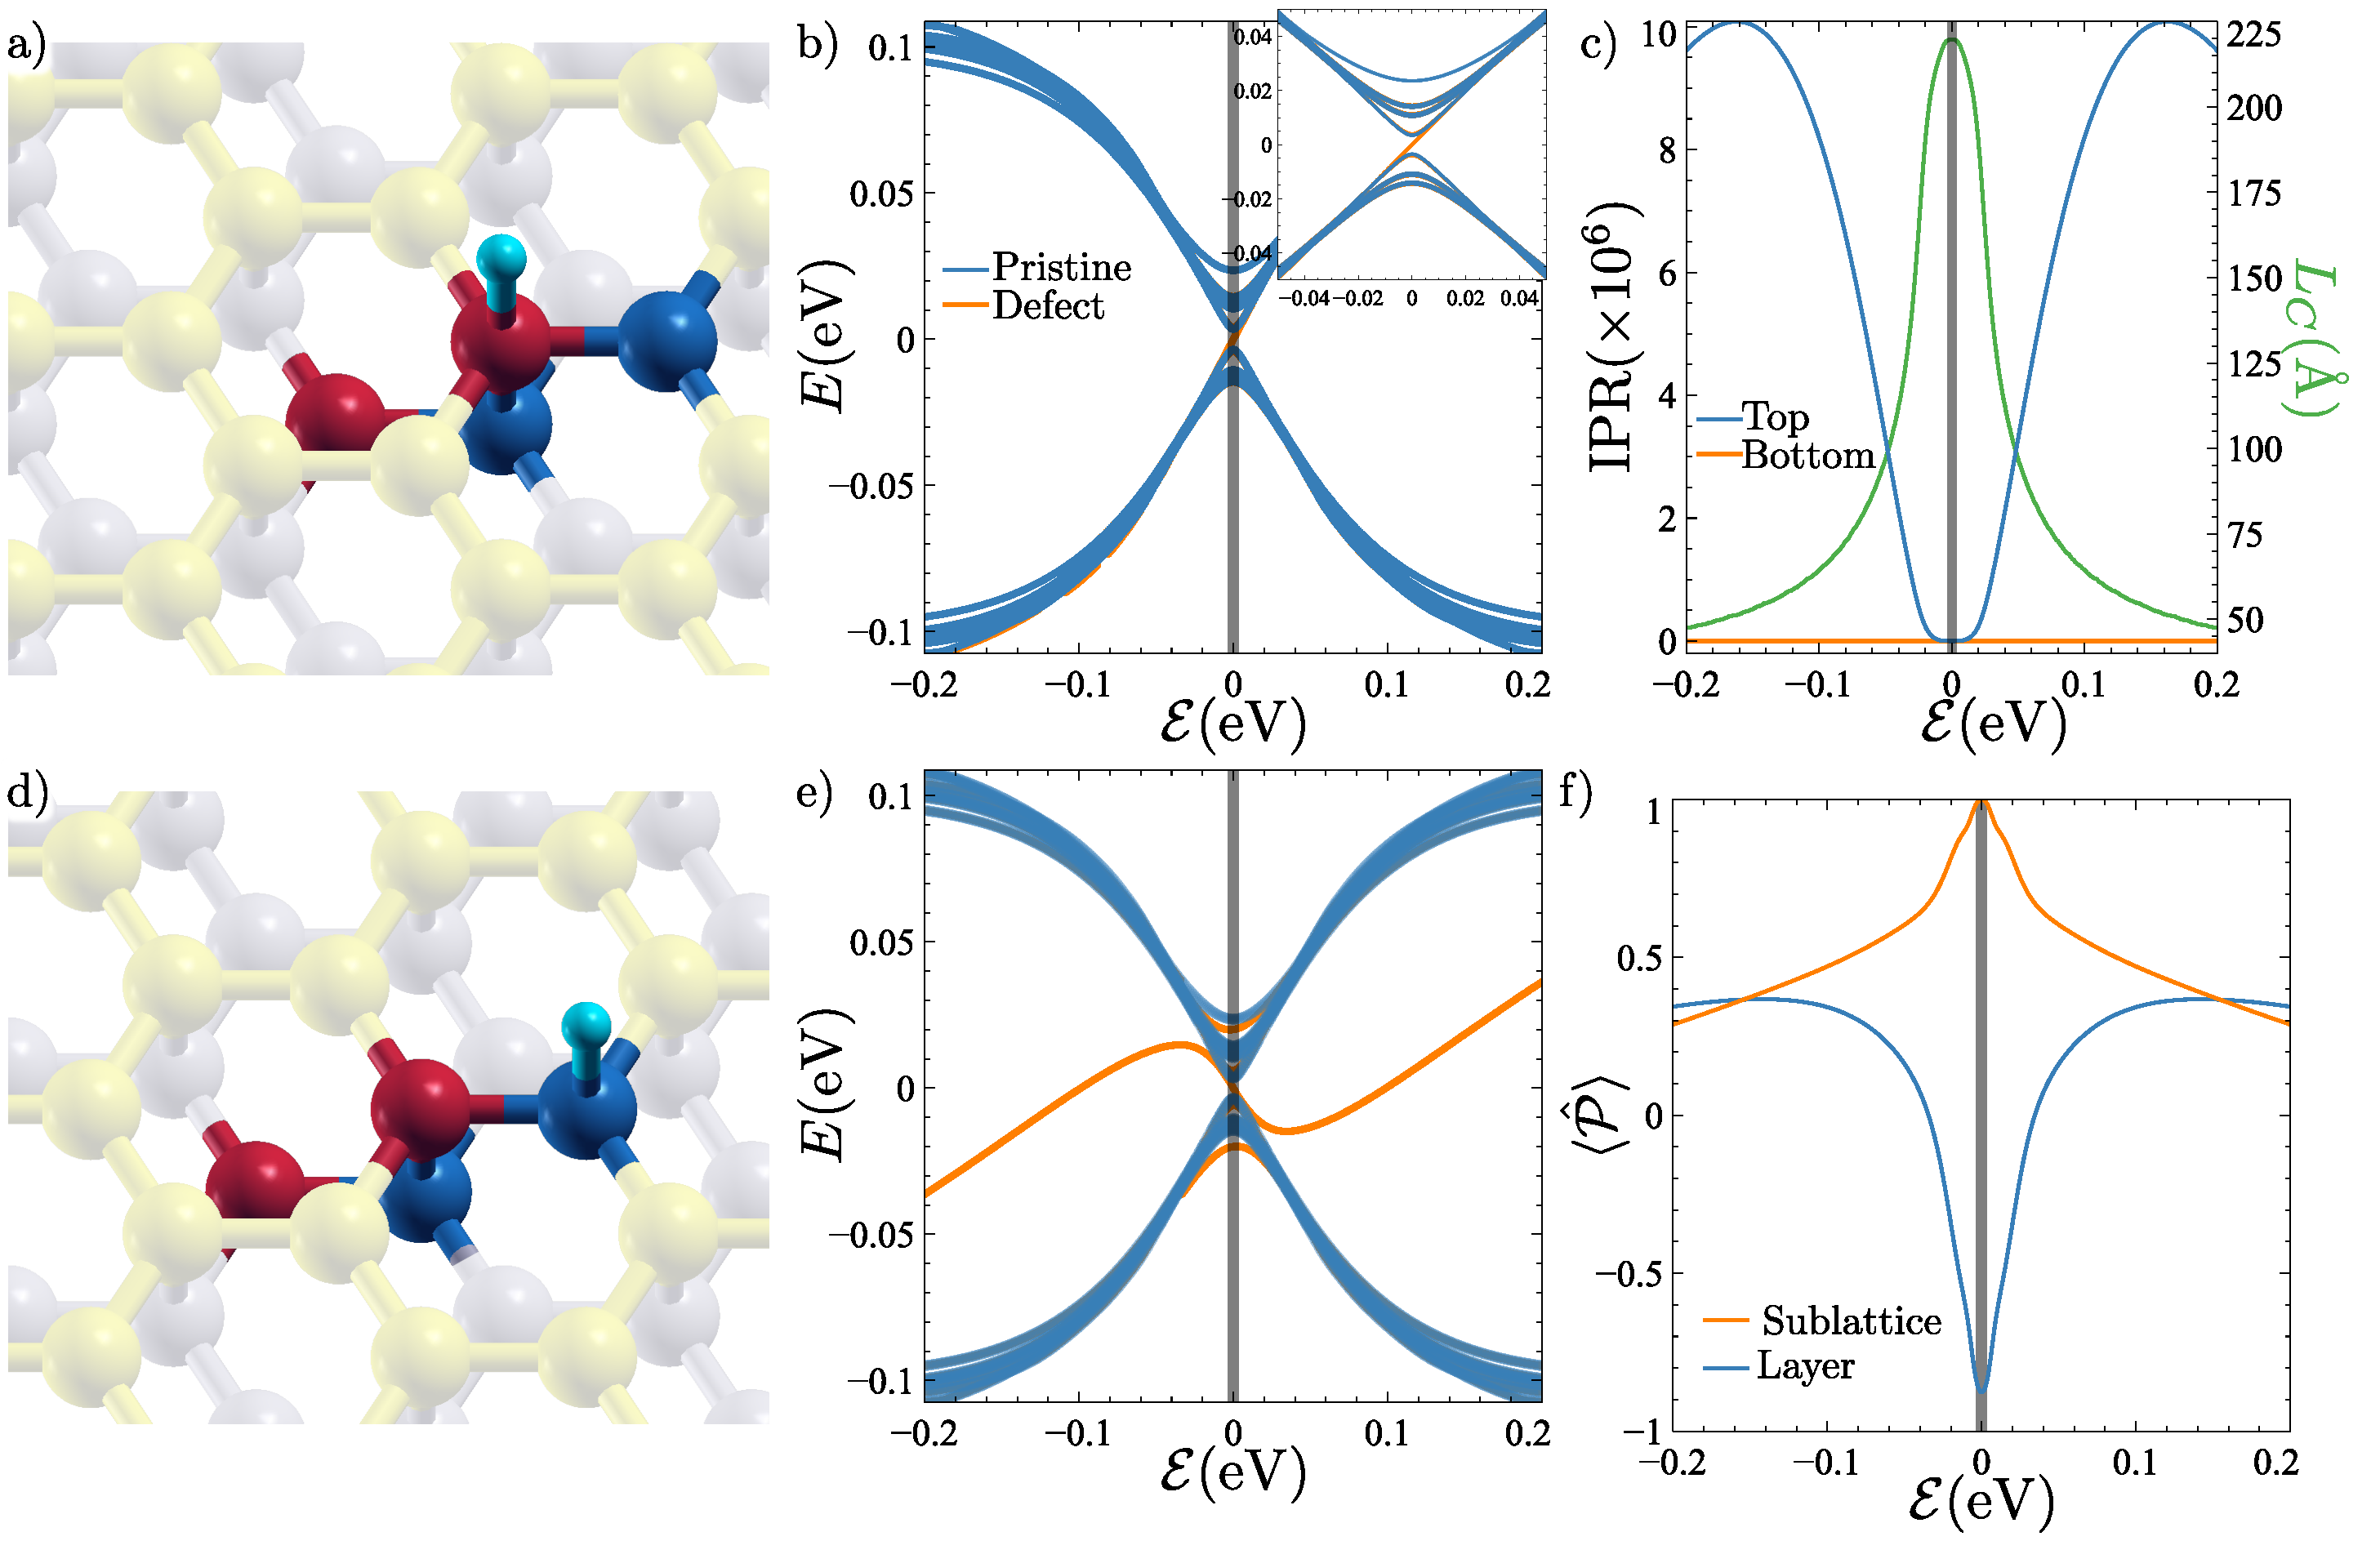
\includegraphics{defects/fig/hollow_connected.pdf}
\vspace{-20pt}
\caption{a,b) Evolution of the spectrum for adatom on a connected site. The in-gap state is shifted directly by the electric field with $100\%$ sublattice and layer polarization, without noticing the bottom layer. Panels c-f) belong to an adatom on a hollow position. e) Evolution of the spectrum with the applied electric field. c) IPR and confinement length dependence on the electric field. f) Evolution of the layer and sublattice polarization as the system loses its bipartite character.}
\label{fig:hollow-connected}
\end{figure}
% \FloatBarrier
%~~~~~~~~~~~~~~~~~~~~~~~~~~~~~~~~~~~~~~~~~~~~~~~~~~~~~~~~~~~%

In each of the layers one of the sublattices is connected to the other layer while the other remains disconnected, with only \emph{intra}-layer interactions. This is, for the bottom layer $A$ atoms are only connected to other atoms in the same layer while in the top layer the $A$ atoms are connected to atoms in both layers.
\medskip

As explored in the previous chapter \ref{ch:vacancy}, the electronic state associated with the introduction of the $sp^3$-defect has most of its weight in the three atoms closest to the defect. That is why the physical character of the two types of defects is so different.

The first option, \fref{fig:hollow-connected}a) is what we call a ``connected'' site (since it is connected to the bottom layer). If the \ce{H} adatom is placed on a connected site, its three closest neighbors are necessarily hollow sites, so the interlayer interactions will not have much effect on them. In fact, for $\mathcal{E}=0$, the electronic state is completely sublattice polarized, hence completely layer polarized\cite{Castro2010} (not shown).
The effect of the electric field on such a state is, in a first approximation, simply a linear shift so the in-gap state quickly gets buried among the rest of the ``continuous'' states as shown in \fref{fig:hollow-connected}b). The physics of the connected sites is explored elsewhere\cite{Castro2010} and we will not study it any further.

% Plots like those of \fref{fig:hollow-connected}b) and e) require a moment to process. Our eyes are way too used to analyze band structures, so it is worth noting that these diagrams are not band structures indeed. They show the evolution of the 9 eigenvalues of the spectrum closest to the Fermi energy. Each ``section'' along the $X$ axis shows the spectrum for a different electric field, $\mathcal{E}$.
\bigskip


The case of placing the adatom on a ``hollow'' site is different. Its first three neighbors are connected sites, so the wave function can hop to the other layer. In fact, \fref{fig:hollow-connected}f) shows that even at $\mathcal{E}=0$ the in-gap state is not $100\%$ layer-polarized, although it is sublattice polarized in agreement with Lieb's theorem.
It will be deeply explained in the following sections, but suffice it to say that, for this configuration, the in-gap state remains inside the gap for any electric field (\fref{fig:hollow-connected}e)) and its extension can be controlled via the electric field (\fref{fig:hollow-connected}c)).
Its localization and composition properties are briefly summarized in plots \fref{fig:hollow-connected}c) and f) for completeness here but we will devote the rest of the thesis to explore it.




\section{A Single defect in graphene bilayer}

From now on we will restrict ourselves to defects on hollow sites.
Diagonalization of a hexagonal island with armchair edges results in a spectrum without states around the Fermi energy. This ``gap'' is solely due to the fact that the system at hand is finite and, in fact, we can see the dependence of such a gap with the size of the system. In figure \fref{confinement}a) we show the incremental procedure used to build bigger islands. The index $N$ is used to label the size of the islands.\footnote{Armchair islands are build based on repetitions of hexagons in the appropriate directions, $N$ is the index describing the number of repetitions. $N=0$ would be like a benzene ring} In order to have a dictionary between the index $N$ and the number of carbon atoms $N_C$ one can use the following relation:
\begin{equation}
   N_C = l\left(18N^2+18N+6\right)
\label{Nc}
\end{equation}
where $l$ labels the layers in the system, $l=2$ represents a bilayer hexagonal island with armchair edges.
The dependence of the gap with the area of the system, proportional to the number of carbon atoms, is nearly linear as shown in \fref{confinement}b) and consequently quadratic with the side of the system as it is expected in a finite quantum system (remember that the energy spectrum of a particle in a well is $E_n\propto n^2/L^2$ being $L$ the size of the well).
%~~~~~~~~~~~~~~~~~~~~~~~~~~ FIGURE ~~~~~~~~~~~~~~~~~~~~~~~~~%
\begin{figure}[!ht!]
\centering
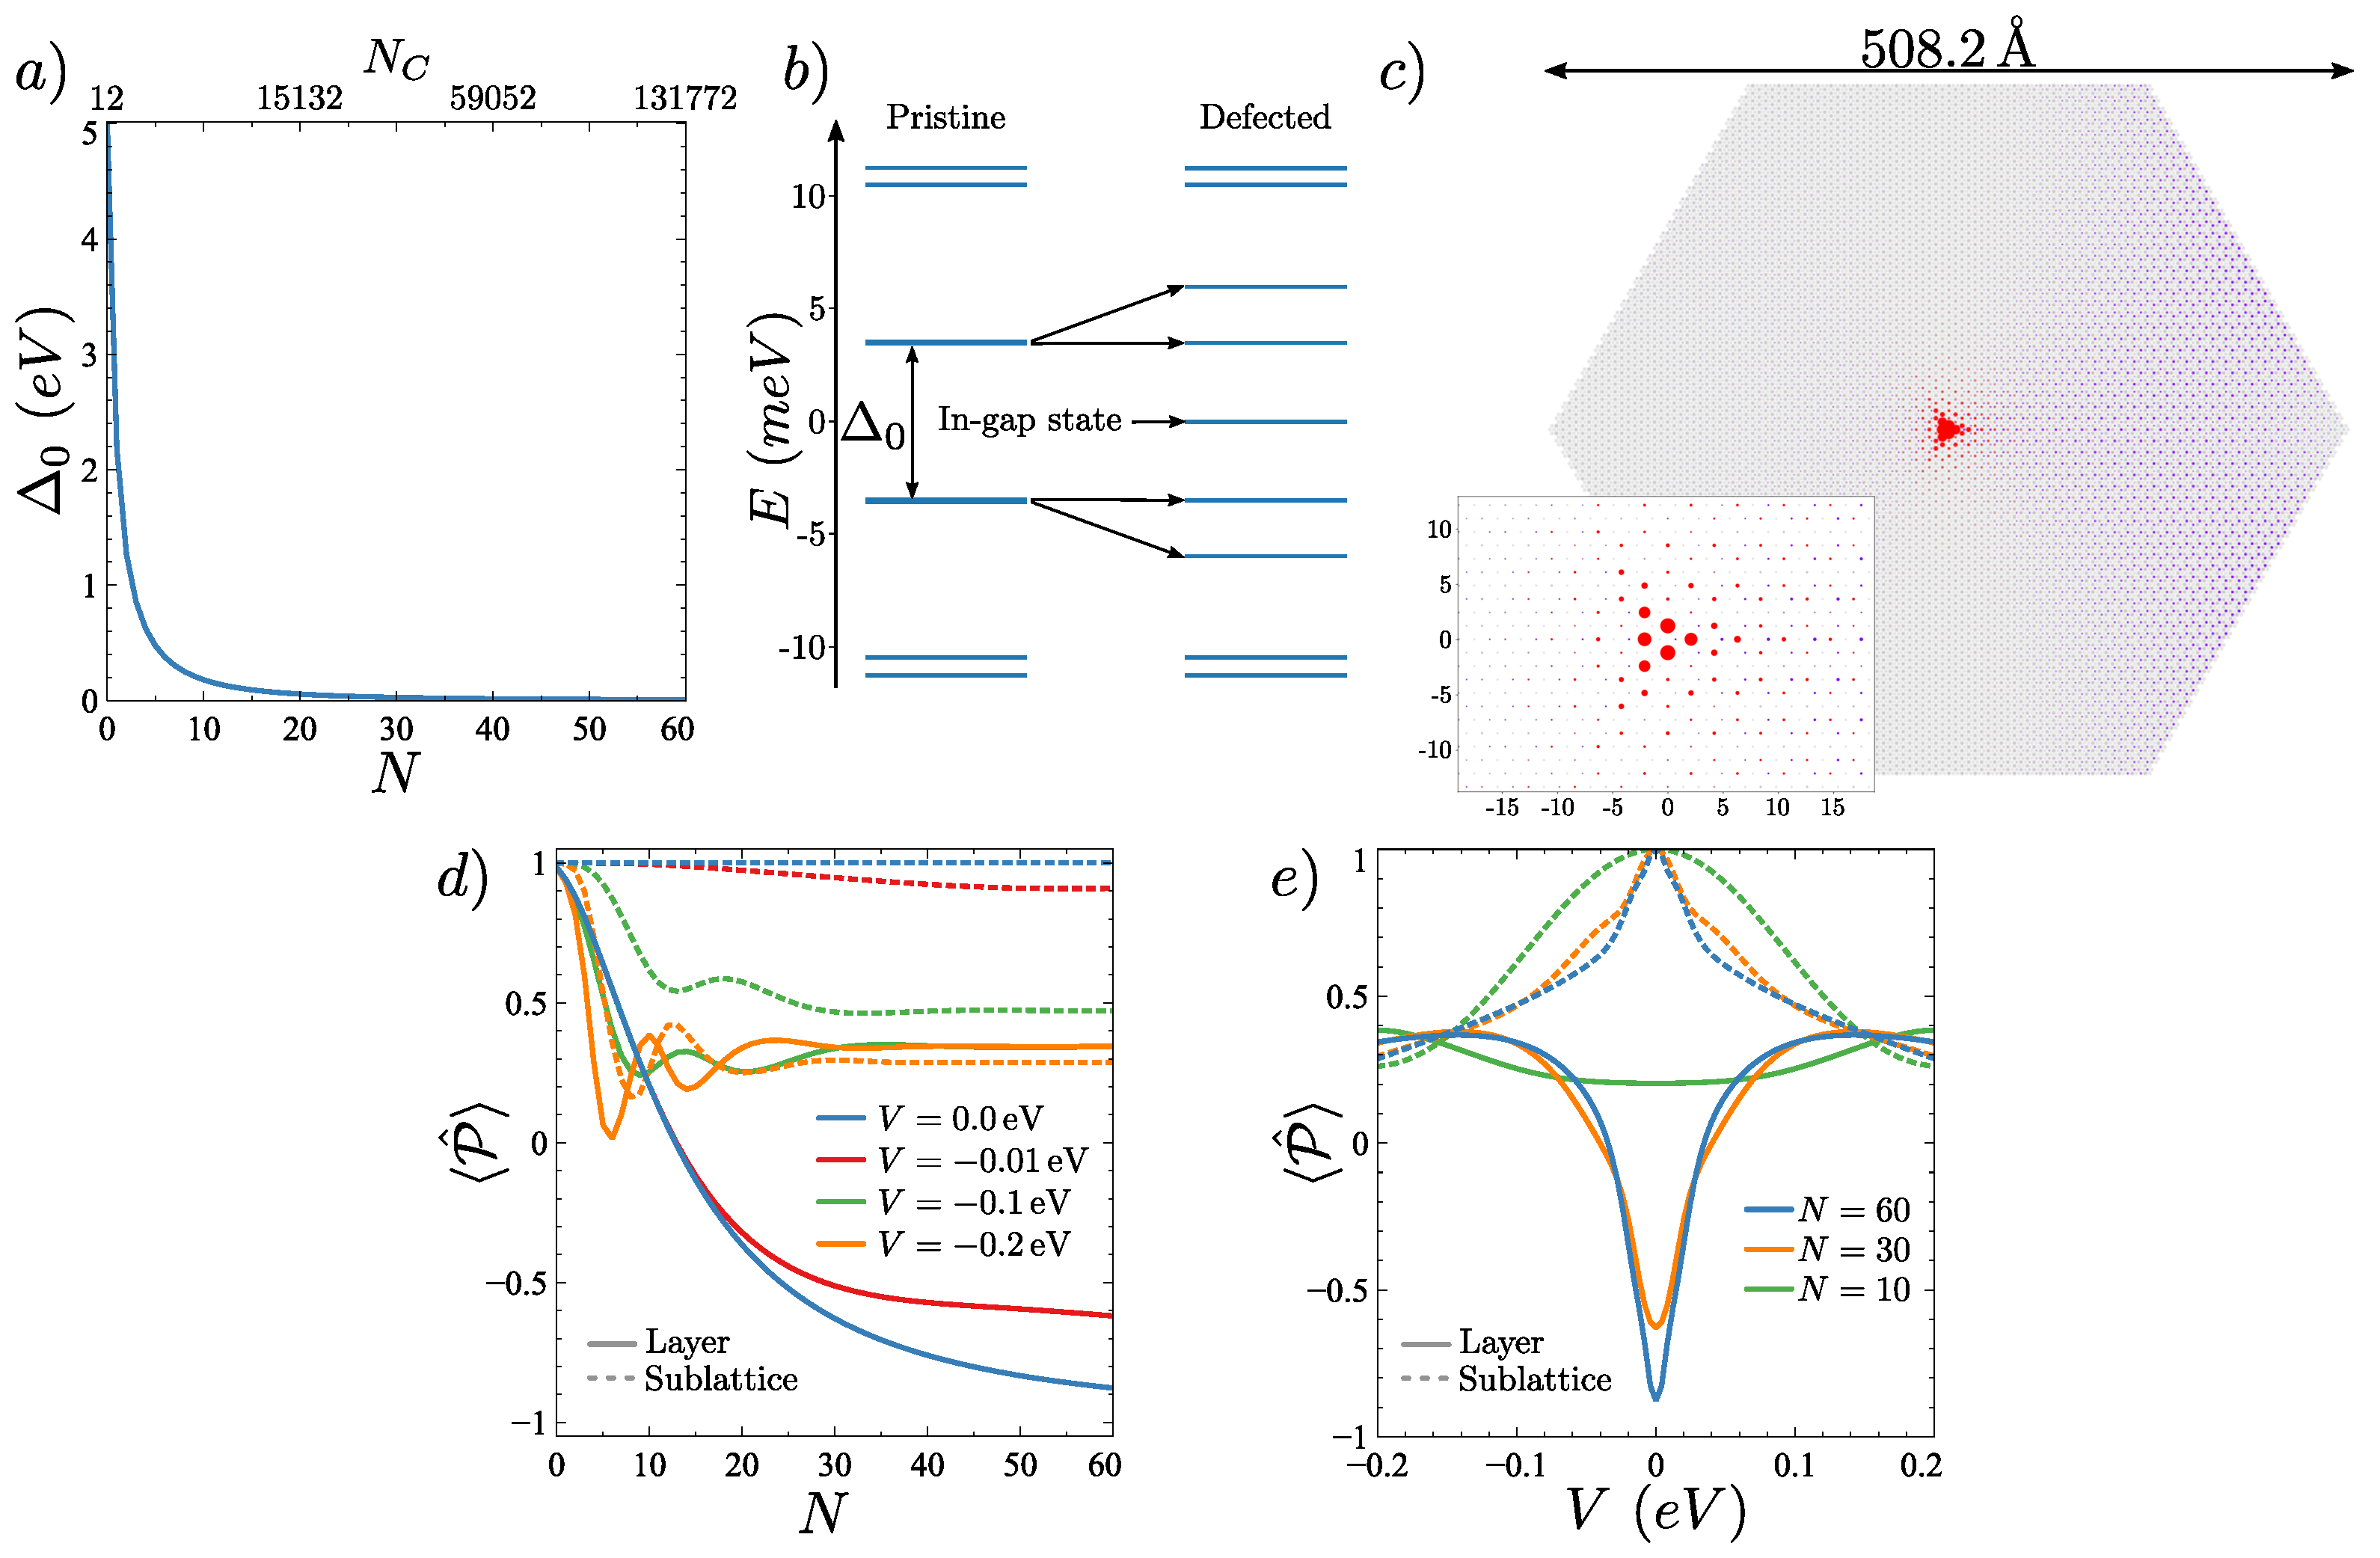
\includegraphics[width=\textwidth]{artlat/fig/confinement.pdf}
\vspace{-20pt}
\caption{$a)$ Scheme of the construction of hexagonal armchair islands, notice the index $N$ labelling the island size. $b)$ Confinement gap as a function of the number of atoms in the island (proportional to the area), biggest island corresponds to $N=60\Rightarrow N_C=131772$ atoms. The gap is almost linear with the area of the island. $c)$ Comparison of a pristine and a defected island, with a vacancy in the central hollow position. An in-gap state appears at zero energy. $d)$ Spatial distribution of the in-gap state. It appears distributed in both the top (red dots) and bottom layer (blue dots). Notice that the state is strongly localized around the vacancy in the top layer (red) while it is spread throughout the bottom layer (blue). The spatial distribution of the bottom layer is affected by the finite size of the sample and its exact shape is but a minor detail. The inset shows a $15\times\SI{10}{\angstrom}$ zoom of the in-gap state around the vacancy. $e)$ Dependence of the layer and sublattice polarizations with the size of the island. $f)$ Evolution of the layer and sublattice polarizations with the electric field for islands of different size.}
\label{confinement}
\end{figure}
% \FloatBarrier
%~~~~~~~~~~~~~~~~~~~~~~~~~~~~~~~~~~~~~~~~~~~~~~~~~~~~~~~~~~~%
\smallskip


The introduction of a $sp^3$-defect creates an in-gap state shown in \fref{confinement}c) without affecting the rest of the spectrum in a significant way. This behavior is completely analogous to the case of monolayer graphene, explored in the previous chapter.

The properties of the in-gap state are explored in the rest of the panels of \fref{confinement}. Panel d) shows the spatial distribution of said state. It is actually quite localized in the top layer (red dots), but completely delocalized over the bottom layer (blue dots).
The particular shape of the distribution of the bottom layer is strongly affected by the edges so it is not to be considered as a reliable result, nevertheless its spreading, calculated later via \ac{ipr}, is consistent through different shapes and island sizes, and in accordance with the literature\cite{Castro2010}.
In the upper layer the in-gap state is very similar to the case of monolayer graphene, the state is mainly distributed among the three closest atoms (it has nearly $C_3$ symmetry, broken just by the finite character of the system) and it decays with the distance as expected.

At $\mathcal{E}=0$ (blue lines in \fref{confinement}e)) Lieb's Theorem guarantees that the in-gap state is sublattice polarized (dashed lines). As the electric field increases, the electronic states tend to mix between the layers which implies also sublattice mixing. As a consequence both the sublattice and layer polarization decrease monotonously.

The layer polarization is a bit tricky to analyze. In the absence of electric field $\mathcal{E}=0$ and for large systems $N\sim60$ the in-gap state shows a strong layer polarization with sign opposed to the layer containing the defect. This behavior is different for smaller samples, completely reversing as $N\to0$. Nonetheless we have to keep in mind that the limit $N\to0$ is clearly out of the scope of this method. For instance, the case $N=0$ is just two benzene rings with an extra \ce{H} on top of one of them; surely the structure and electronic distribution, for this situation will not be correctly captured by a \ac{tb} model. We only include this limit here for completeness.
Non-monotonous behavior is observed for smaller islands, say $N<30$ possibly as a consequence, again, of the finite size effects, but for larger islands the results become stable and independent of the system size.

It is worth noting that ``big'' or ``small'' in this system depends on the applied electric field. In the limit $\mathcal{E}=0$ the in-gap state is so delocalized that in order to recover the expected behavior of infinite bilayer graphene we would require an infinite island. In opposition, for strong $\mathcal{E}$, the in-gap state becomes localized within a certain radius. In this situation ``big'' only means bigger than that radius.


Finally, \fref{confinement}e) shows the layer and sublattice polarization of the in-gap state for different sizes of the island as a function of the electric field. Naturally for low electric fields $\mathcal{E}\to0$ there will be a big difference depending on the size of the island. At $\mathcal{E}=0$ the in-gap state is spread all over the sample resulting in $100\%$ sublattice polarization (Lieb's Theorem) and a certain layer polarization depending on the island size. The results seems to indicate that the layer polarization, $\langle\hat{L}\rangle\to\pm1$ as the island size goes to infinite. For strong electric fields the results beyond $N=30$ converge quickly.




%   %\newpage
%   %AAAAAAAAAAAAAAAAAAAAAAAAAAAAAAAAA
%   %\newpage
%   %Namely in each of the layers one of the sublattices is connected to the other layer while the other remains disconnected, only with \emph{intra}-layer interactions. This is, for the bottom layer A atoms are only connected to other atoms in the same layer while the A toms in the top layer are connected to atoms in the bottom layer as well.
%   %% Since deposition of atomic \ce{H} has been demonstrated with atomic precision\cite{Brihuega2016}, we can afford the luxury of restraining ourselves to a particular kind of defect.
%   
%   
%   
%   %%%% XXX
%   %%%%   \section{A note on the geometry}
%   %%%%   %All the vacancies considered will always be chosen on a hollow position (see fig~\ref{geo_sketch} $c)$) even if it not specified in the text. The behavior of vacancies in connected sites is studied somewhere else\cite{Castro2010}.
%   %%%%   
%   %%%%   When only one vacancy is considered, it will be placed at the hollow atomic position closest to the center of the island in order to maximize the distance to the edges.
%   %%%%   
%   %%%%   When two vacancies are considered, they will be placed as separated as possible from the edges, as shown in \fref{geo_sketch}b). This configuration (rather than placing one in the center, for instance) allows the study of a wider range for both, the angle $\alpha$ and distance $d$.
%   %%%%   % When more than two vacancies are considered, they will be placed in the vertices of a regular polygon centered in the island.
%   %%%%   
%   %%%%   % XXX For later, when talking about the angle
%   %%%%   % Note that as long as the border effects are negligible, and due to the $C_3$ symmetry of the in-gap states in graphene, we only need to explore the range of angles between vacancies of $\alpha\in\left[0,60\right]$.
%   %%%%   
%   %%%%   %~~~~~~~~~~~~~~~~~~~~~~~~~~ FIGURE ~~~~~~~~~~~~~~~~~~~~~~~~~%
%   %%%%   \begin{figure}[h!]
%   %%%%   \centering
%   %%%%   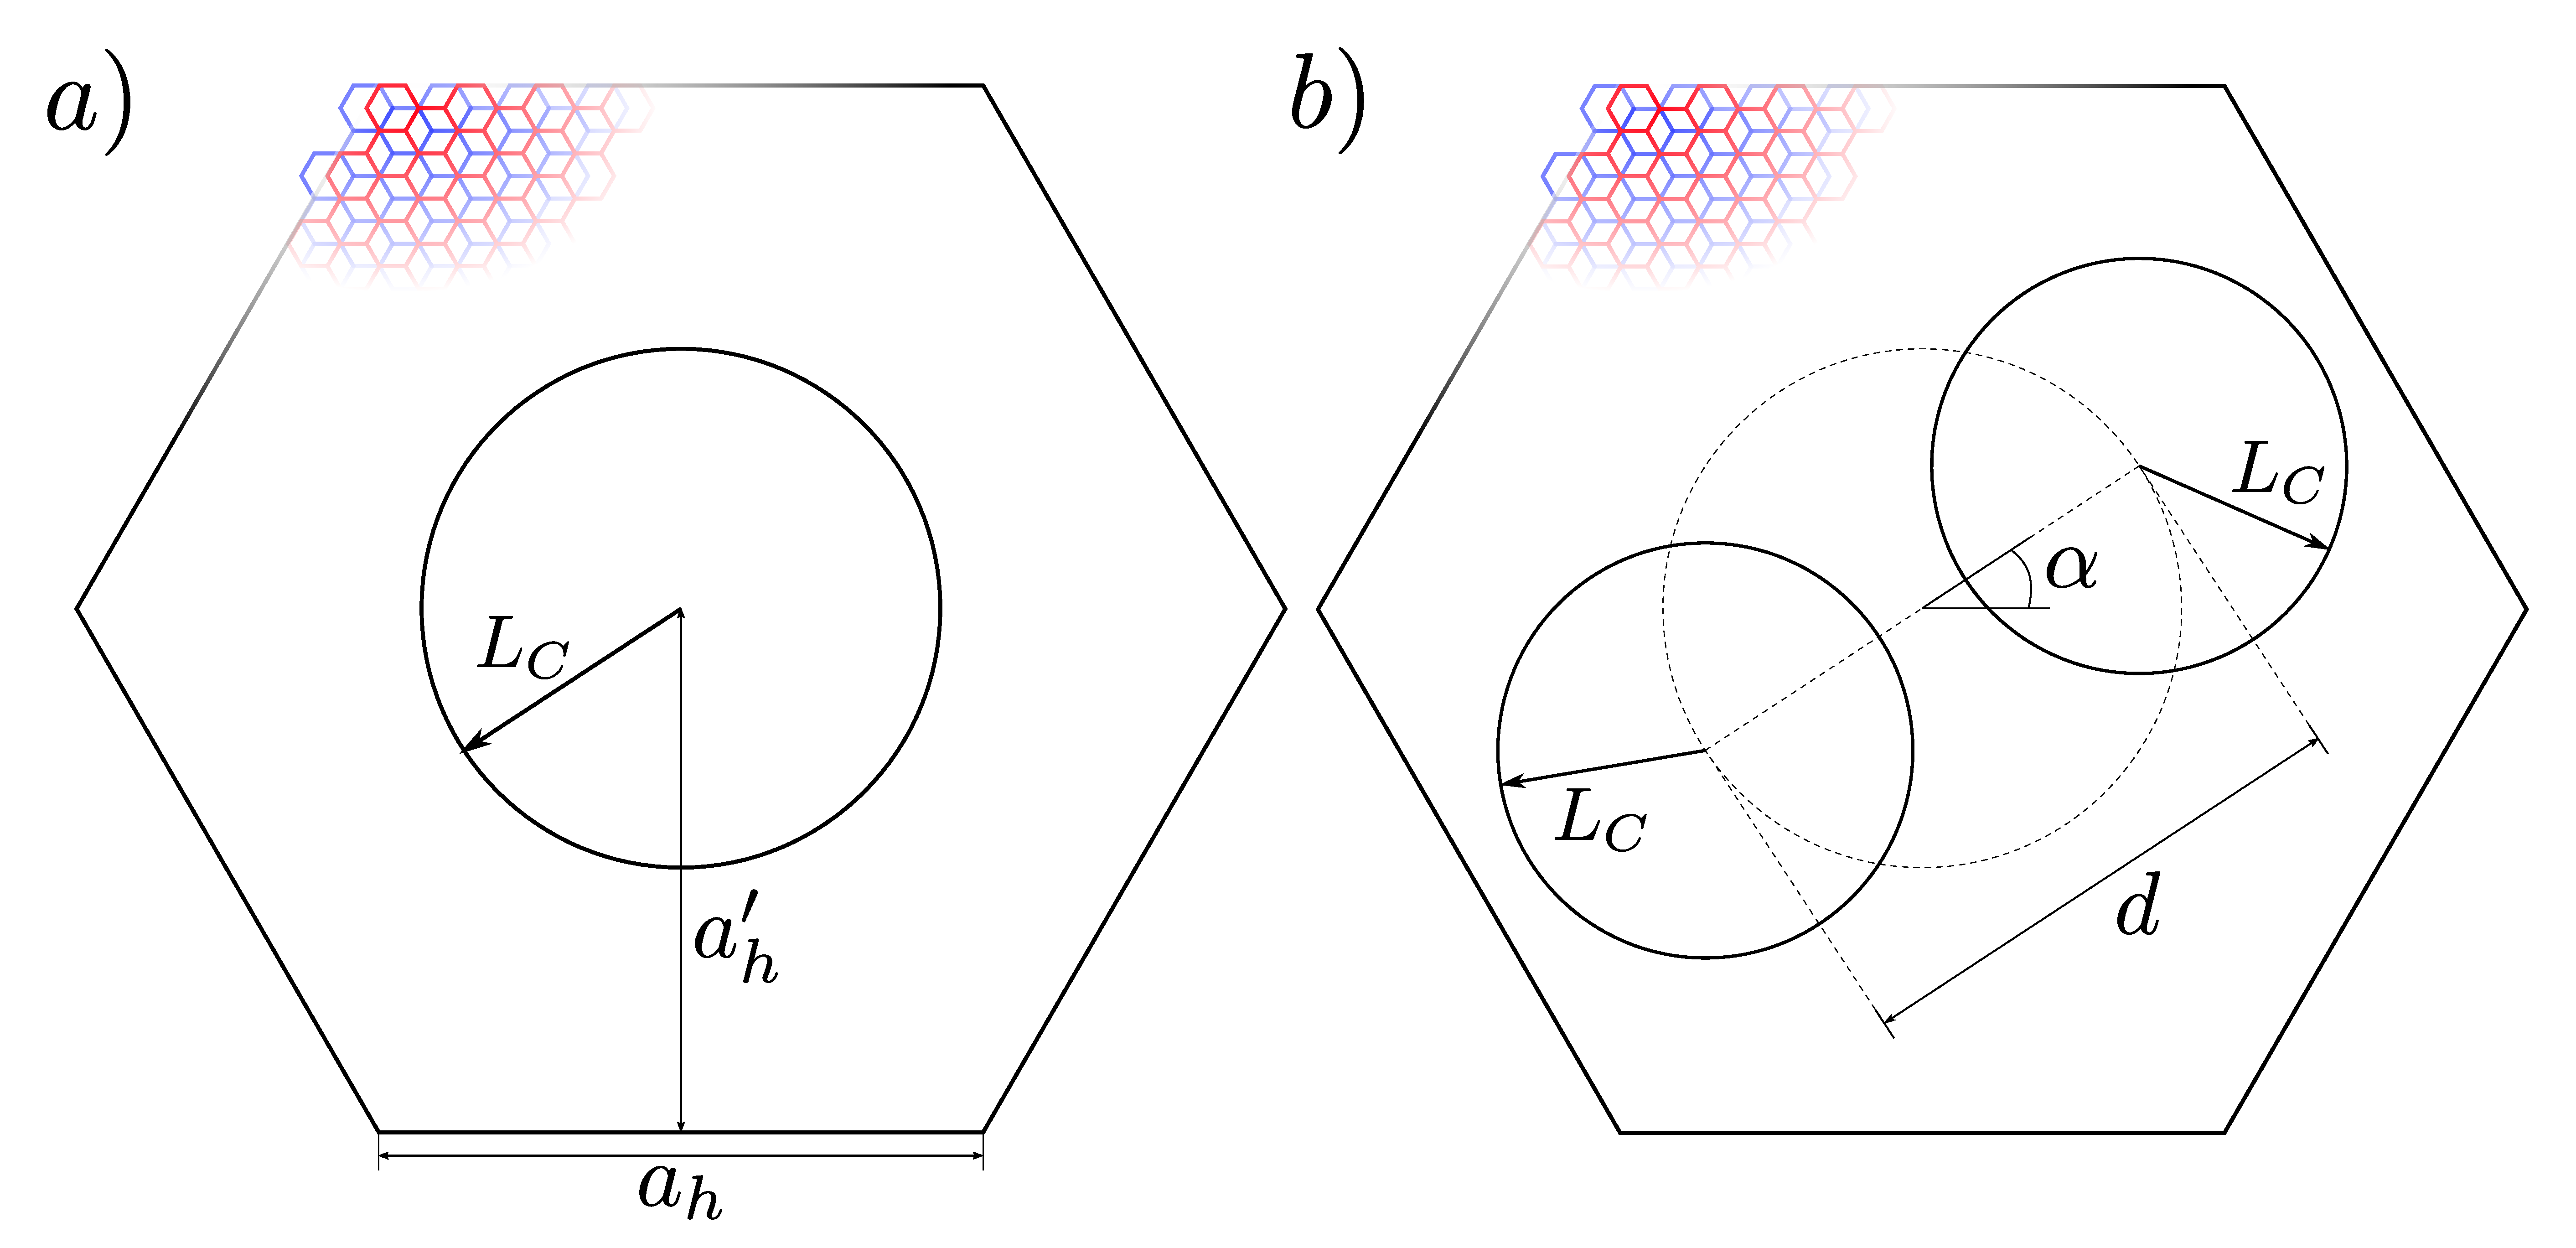
\includegraphics[width=0.7\textwidth]{artlat/fig/vacs_sketch.pdf}
%   %%%%   \vspace{-10pt}
%   %%%%   \caption{$a)$ and $b)$ show sketches of the position of the vacancies and relevant geometric information. In the upper left corner the real atomic structure is shown using blue for the lower layer and red for the upper one. The length $L_C$, defined later in the text, is the typical size of the in-gap state.} % $c$ atomic structure showing the ``connected'' and ``hollow'' sites in the upper layer as well as the $A/B$ sublattices (in red/blue).}
%   %%%%   \label{geo_sketch}
%   %%%%   \end{figure}
%   %%%%   % \FloatBarrier
%   %%%%   %~~~~~~~~~~~~~~~~~~~~~~~~~~~~~~~~~~~~~~~~~~~~~~~~~~~~~~~~~~~%
%   %%%%   
%   %%%%   % In the case of graphene monolayer, every atomic position is equivalent, so regardless of the position in which the adatom is introduced, the physical effect will be the same.
%   %%%%   % This is not the case for $AB$-stacked bilayer graphene. In each layer one of the sublattices is connected to atoms of the other layer, while the other sublattice lays on hollow spaces.
%   
%   
%   %So, for infinite bilayer graphene there are two inequivalent sites to place an adatom in AB-stacked bilayer graphene, depicted in \fref{fig:hollow-connected}a), d).
%   %% shown in \fref{fig:hollow-connected}a) and d). 
%   %Depending on where the $sp^3$ defect is placed, we will refer to them as being in a ``connected'' (a)) or a ``hollow'' site (d)).
%   
%   %As explored in the previous chapter \ref{ch:vacancy}, the electronic state associated with the introduction of the $sp^3$-defect has most of its weight in the three closest atoms.
%   %If the \ce{H} adatom is placed on a connected site, its three closest neighbors are necessarily hollow atoms, so the interlayer interactions will not have much effect on them. In fact, for $\mathcal{E}==0$, the state electronic state is completely sublattice polarized, hence completely layer polarized.
%   %The effect of the electric field on such a state is, in a first approximation, simply a linear shift so the in-gap state quickly gets buried among the rest of the ``continuous'' states. The physics of the connected sites is explored elsewhere\cite{Castro2010} and we will not study it any further.
%   
%   %The case of placing the adatom on hollow site is different and we will explore it in detail.
%   
%   %%~~~~~~~~~~~~~~~~~~~~~~~~~~ FIGURE ~~~~~~~~~~~~~~~~~~~~~~~~~%
%   %\begin{figure}[h!]
%   %\centering
%   %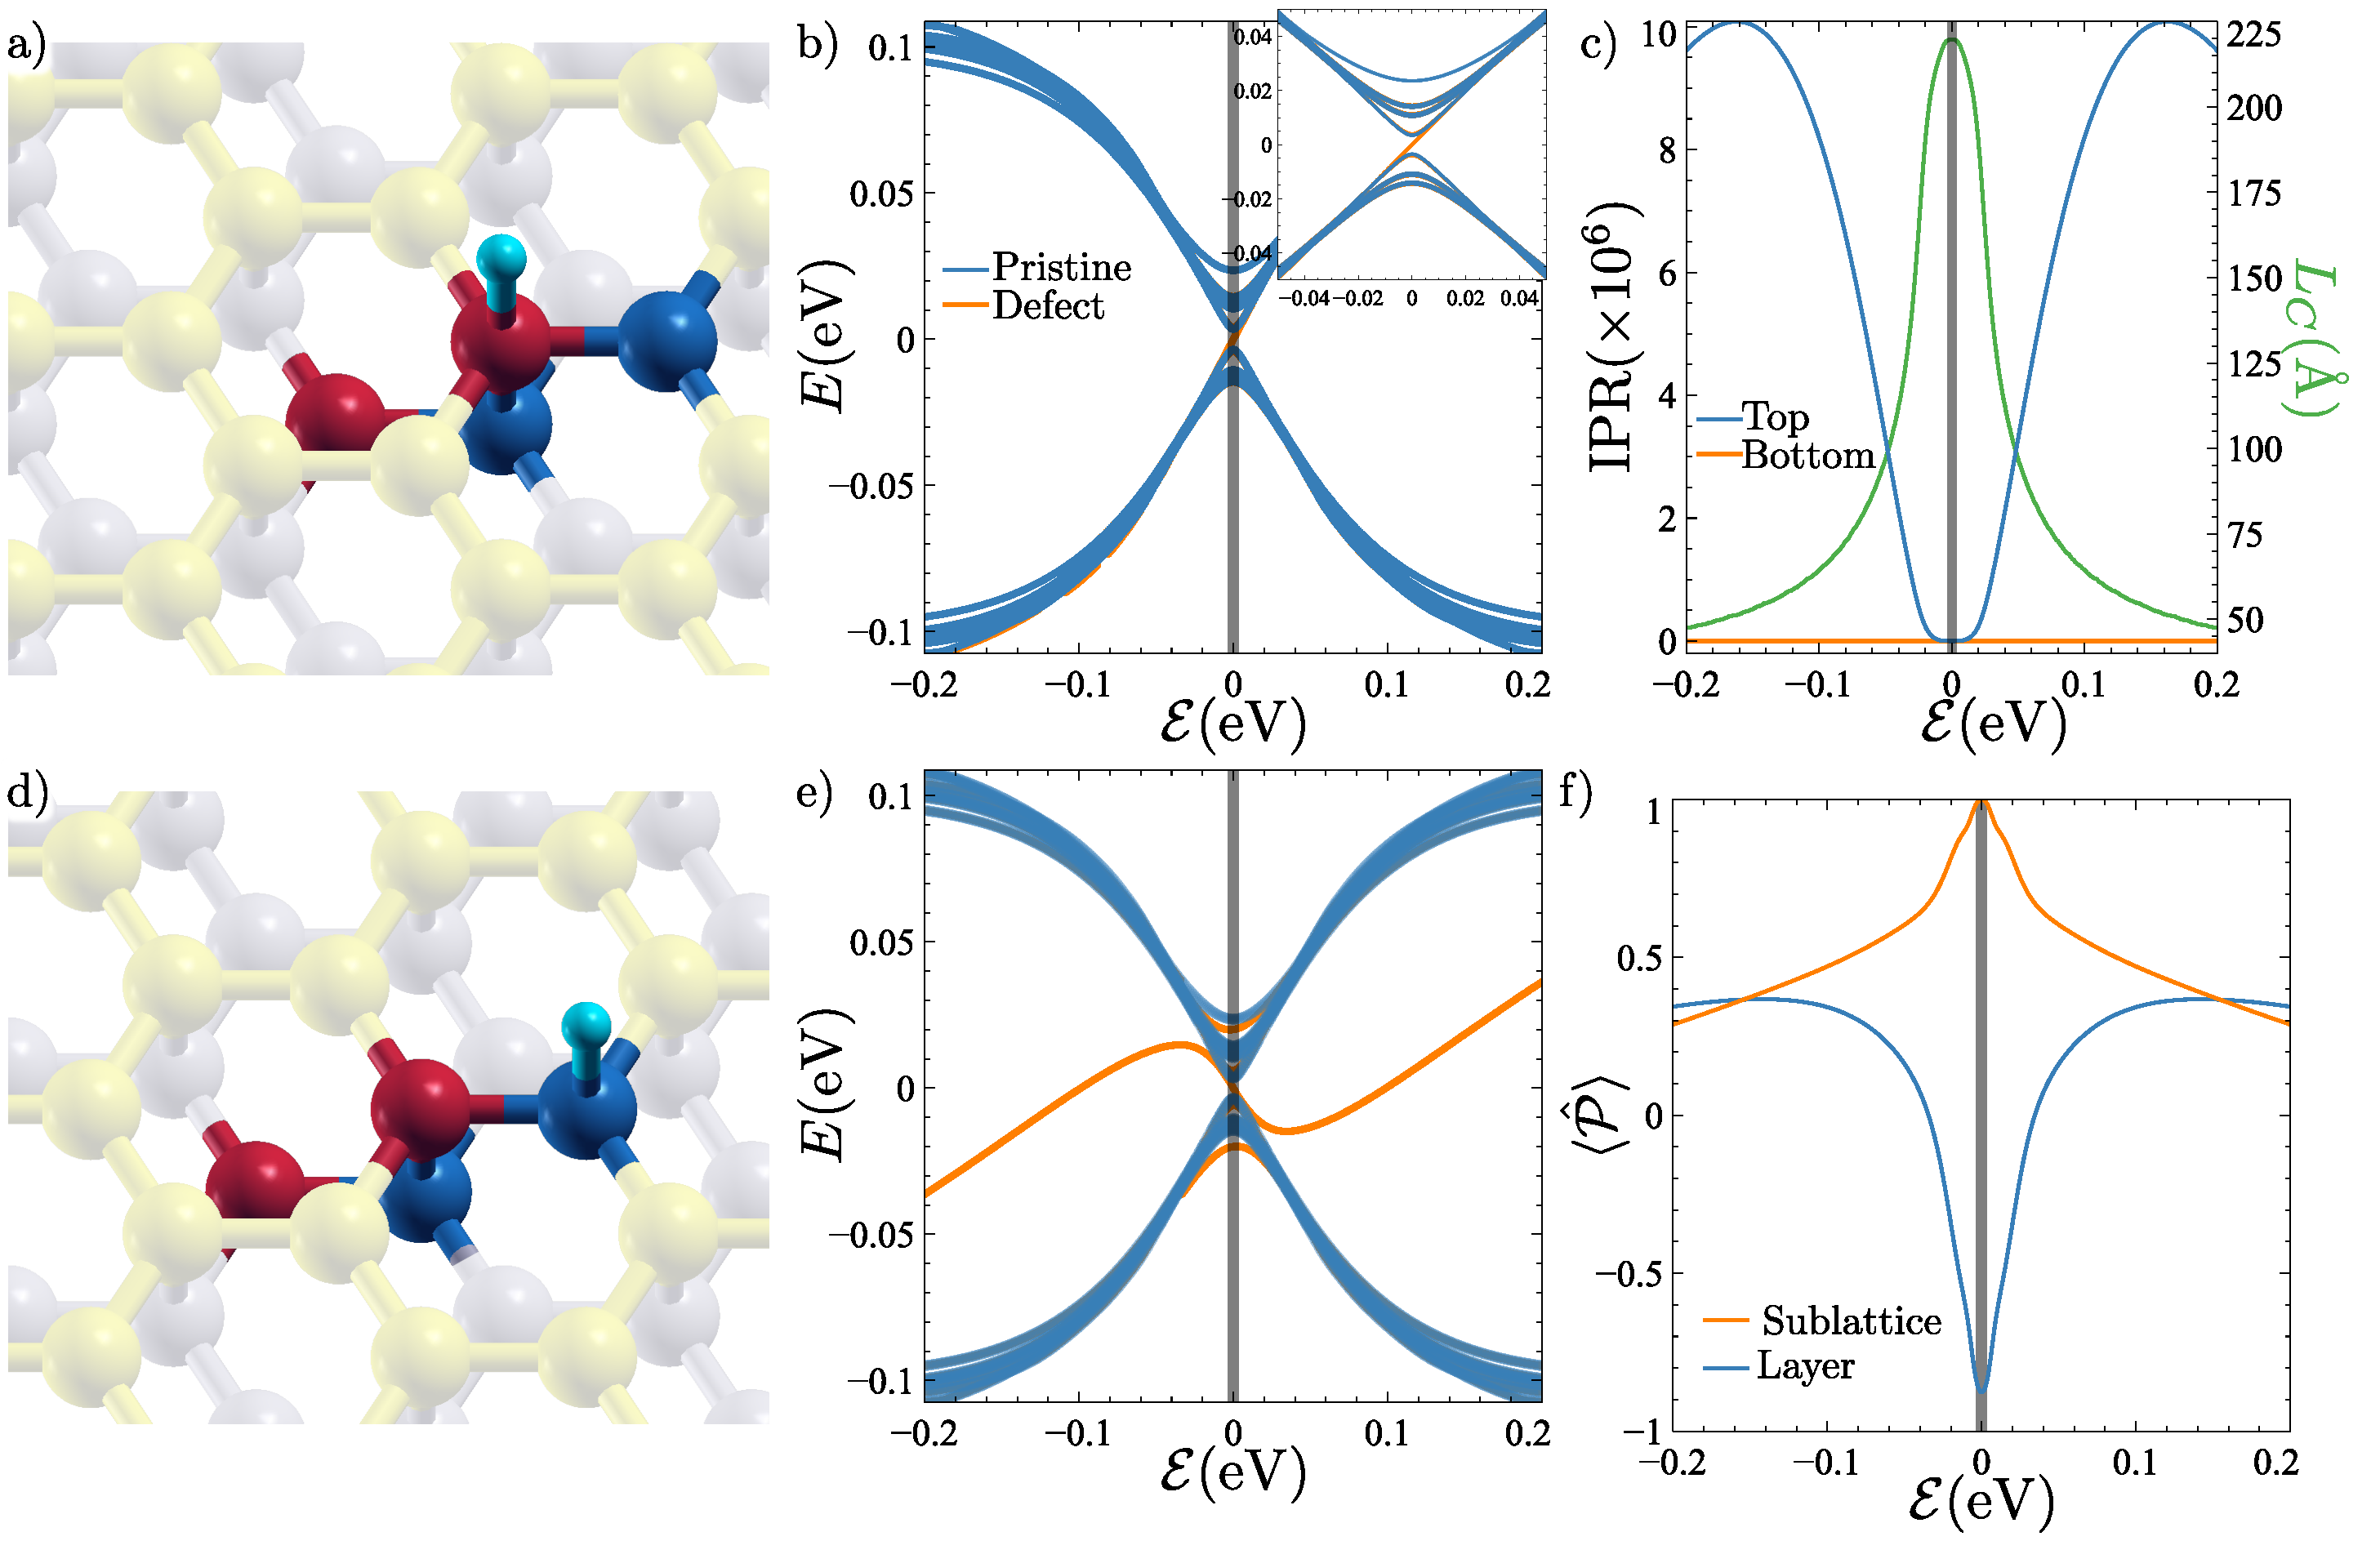
\includegraphics{defects/fig/hollow_connected.pdf}
%   %\vspace{-20pt}
%   %\caption{a,b) Evolution of the spectrum for adatom on a connected site. The in-gap state is shifted directly by the electric field with $100\%$ sublattice and layer polarization, without noticing the bottom layer. Panels c-f) belong to an adatom on a hollow position. e) Evolution of the spectrum with the applied electric field. c) IPR and confinement length dependence on the electric field. f) Evolution of the layer and sublattice polarization as the system loses its bipartite character.}
%   %\label{fig:hollow-connected}
%   %\end{figure}
%   %% \FloatBarrier
%   %%~~~~~~~~~~~~~~~~~~~~~~~~~~~~~~~~~~~~~~~~~~~~~~~~~~~~~~~~~~~%
%   
%   %\section{The finite system}
%   %When a single vacancy is placed in graphene bilayer (or graphene, for that matter), the translational invariance is broken, so its description in terms of Bloch functions is not possible. In the previous chapter we introduced an embedding technique (see \ref{sec:GF}) that provides a workaround in which we consider the defective part of the system to be restricted to a limited region while the rest of the system remains pristine.
%   %This approach is quite computationally expensive and, while it provides a way to calculate the Green's function, it is not possible to obtain the wave function which will be necessary later on.
%   
%   %In order to retain the wave function information we are going to consider a huge but finite hexagonal island with armchair edges. We chose the island to have armchair edges in order to avoid the edge states at the Dirac point present in systems with zig-zag edges.\cite{Nakada1996}
%   %%We will consider a big enough island so we can neglect the edge effects.
%   %The largest island will be $\SI{50.6}{\nm}$ in diameter, containing 131772 atoms\footnote{This limit is based solely upon RAM and patience, it would be feasible to keep increasing it.}.  % limit RAM-patience
%   
%   
%   %Such a system will be our playground to explore the behavior of a single vacancy when an external electric field is applied. Since we are dealing with a finite system, it is expected to present a confinement gap.
%   %This gap decreases linearly with the area of the island (quadratically with the side) as shown in \fref{confinement}a).
%   %\smallskip
%   
%   %It is worth noting that this model is doomed to break down when the scale of the electric field is comparable to the confinement gap. In the limit of zero electric field $\mathcal{E}\to 0$, ideally we would like to recover completely delocalized states on the $p_z$-manifold as it is the case of infinite bilayer graphene. Nonetheless, the finite size of the system do not allow that, so the edges become really important for the description of the system.
%   %Since our goal is to study defects in bilayer graphene, we shall stay clear of the small electric field regime in order to avoid finite size effects.
%   %%Depending on the calculation different sizes for the island can be chosen with no major consequences.
%   %%~~~~~~~~~~~~~~~~~~~~~~~~~~ FIGURE ~~~~~~~~~~~~~~~~~~~~~~~~~%
%   %\begin{figure}[!ht!]
%   %\centering
%   %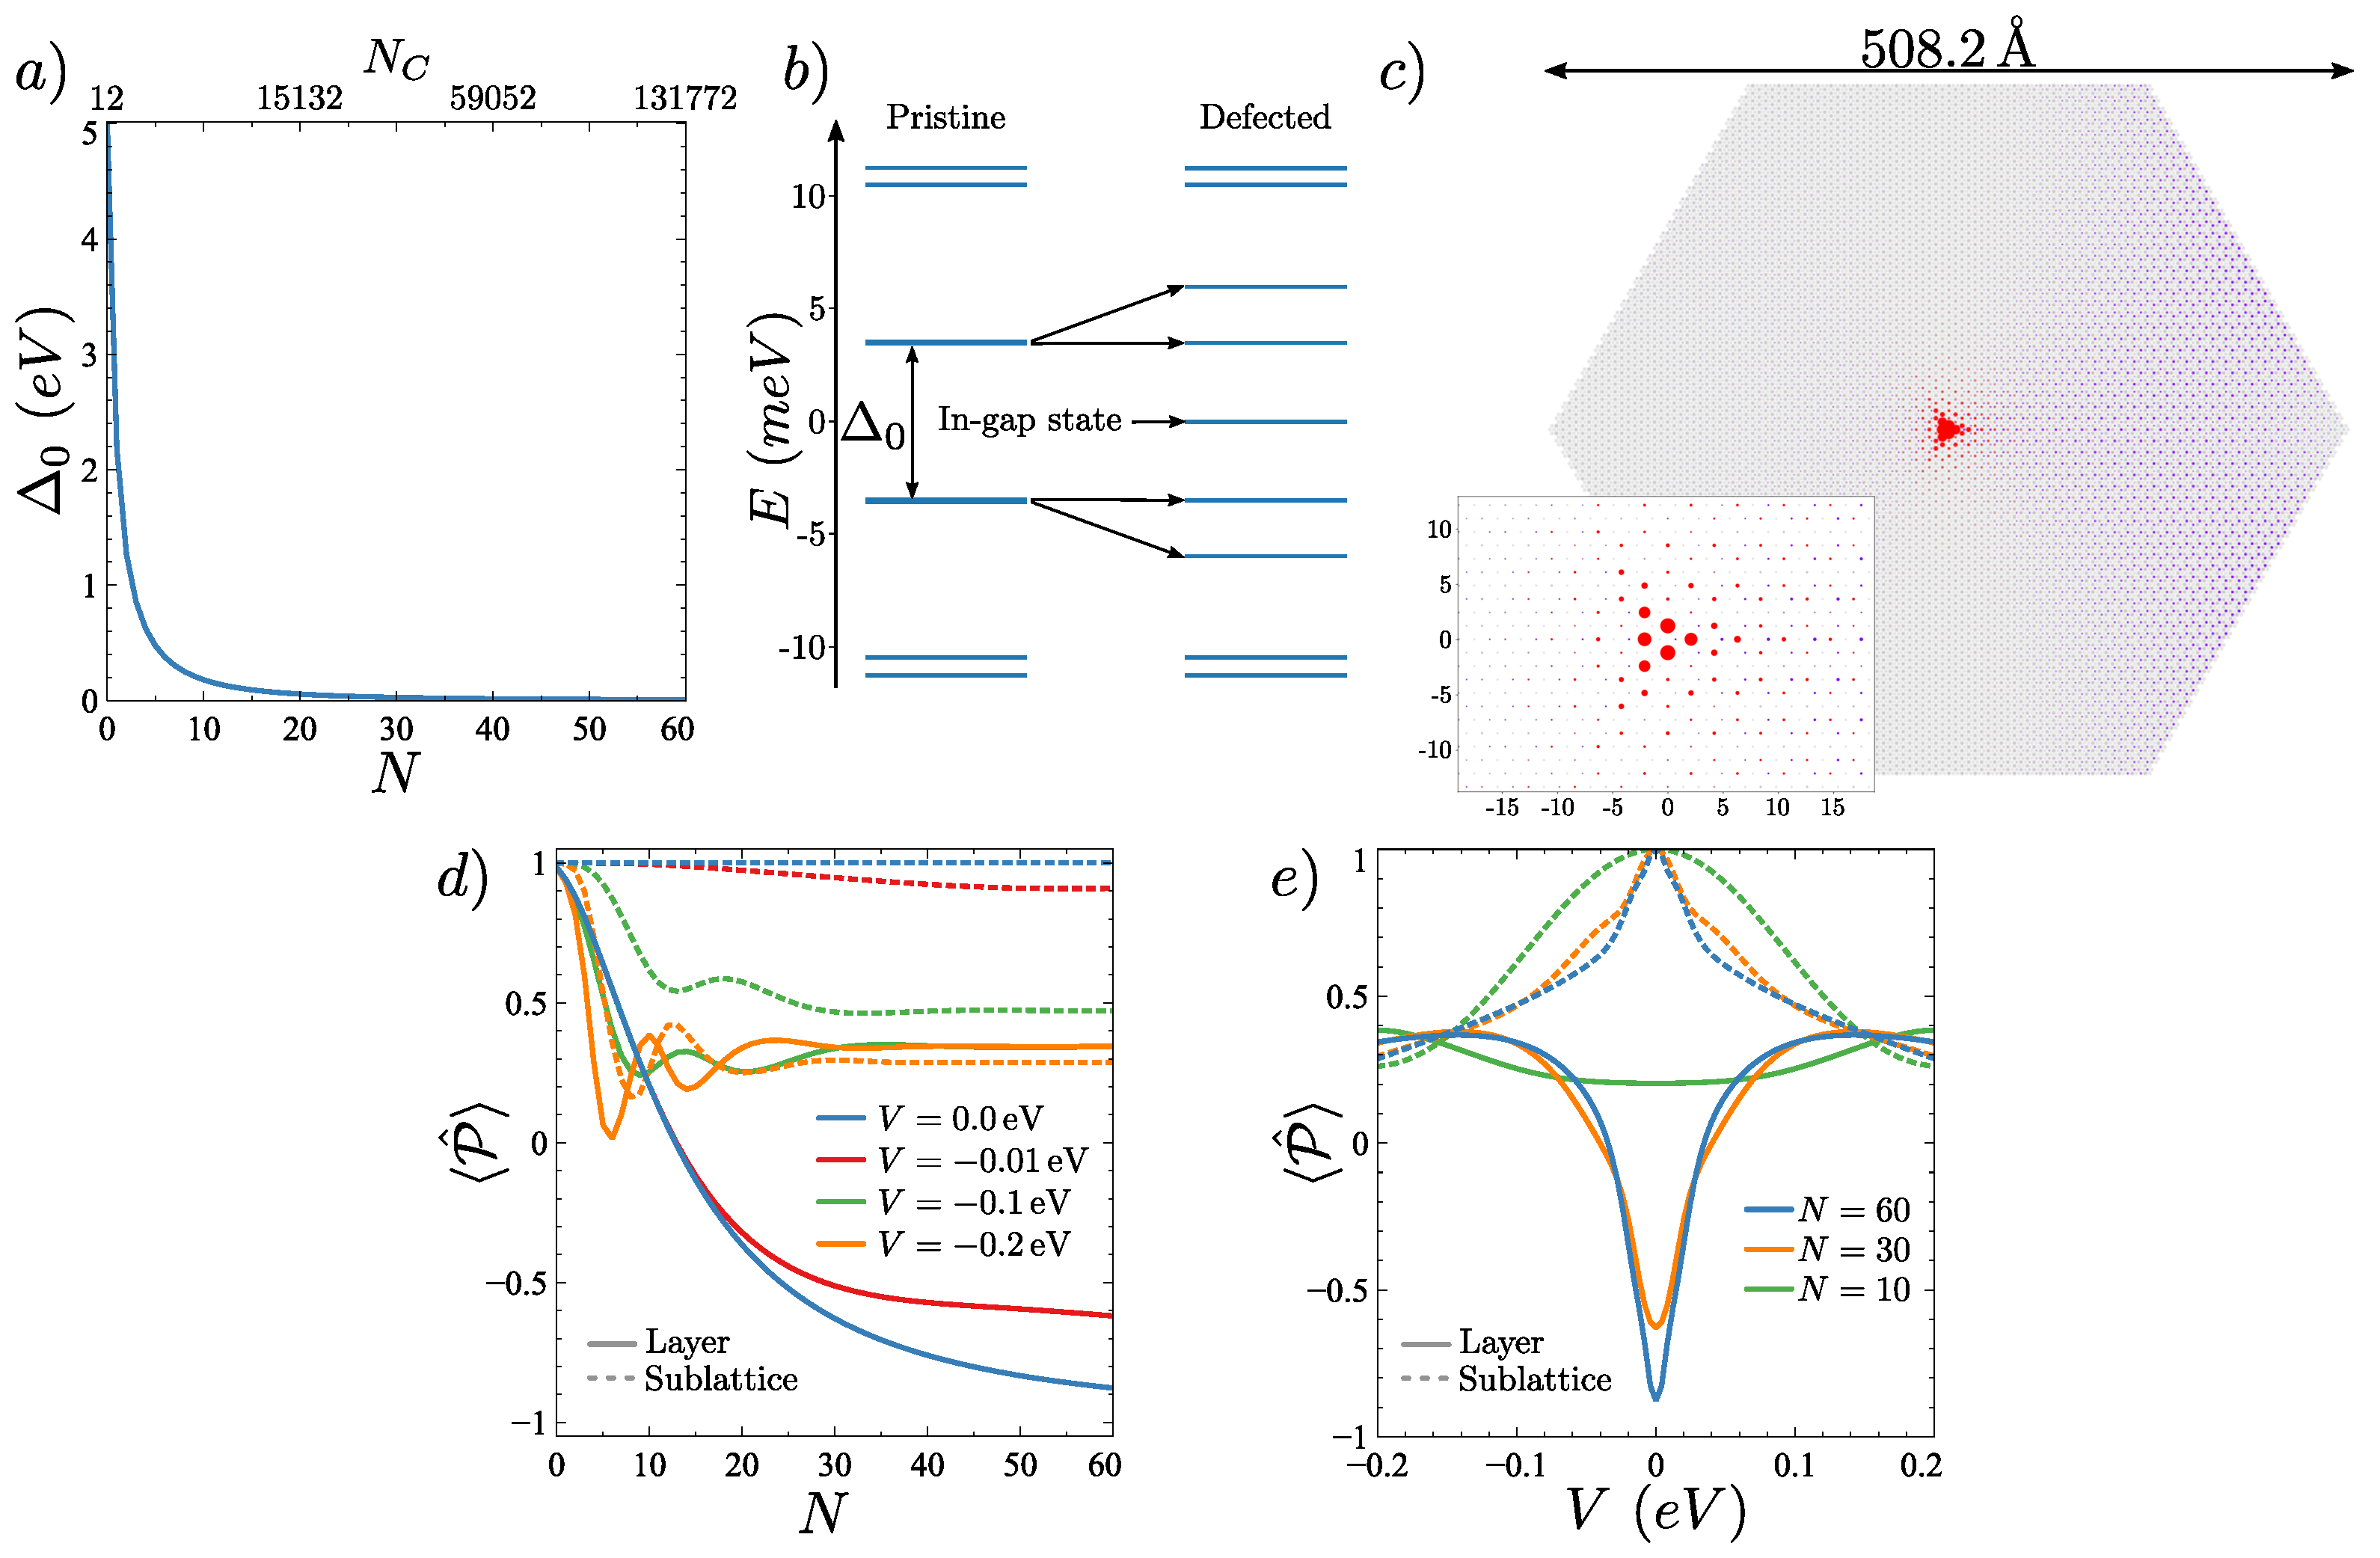
\includegraphics[width=\textwidth]{artlat/fig/confinement.pdf}
%   %\vspace{-20pt}
%   %\caption{$a)$ Confinement gap as a function of the size of the island (lower axis) and the number of carbon atoms $N_C$ in the island (upper axis). $b)$ Comparison of a pristine and a defected island, with a vacancy in the central hollow position. An in-gap state appears at zero energy. $c)$ Spatial distribution of the in-gap state. It appears distributed in both the top (red dots) and bottom layer (blue dots). Notice that the state is strongly localized around the vacancy in the top layer (red) while it is spread throughout the bottom layer (blue). The spatial distribution of the bottom layer is affected by the finite size of the sample and its exact shape is but a minor detail. The inset shows a $15\times\SI{10}{\angstrom}$ zoom of the in-gap state around the vacancy. $d)$ Dependence of the layer and sublattice polarizations with the size of the island. $e)$ Evolution of the layer and sublattice polarizations with the electric field for islands of different size.}
%   %\label{confinement}
%   %\end{figure}
%   %% \FloatBarrier
%   %%~~~~~~~~~~~~~~~~~~~~~~~~~~~~~~~~~~~~~~~~~~~~~~~~~~~~~~~~~~~%
%   
%   
%   %\section{The finite system}
%   %Since we are going to use a finite system  there will not be band dispersions to discuss but rather we will focus on the inspection of discrete spectrums.
%   %We can calculate the spectrum of the system with and without a vacancy in order to compare both of them. Of course the full diagonalization of a $131772\times131772$ Hamiltonian is, at the very least, challenging for any standard computer, so we will use Lanczos diagonalization\cite{Lanczos1950, Ojalvo1970, Arnoldi1951} to obtain only the 9 eigenvalues closest to the Fermi energy\footnote{The number of eigenvalues to obtain is arbitrary although Lanczos diagonalization is better suited, and efficient, for a small number of them}.
%   
%   %In such a huge system there are as many states are sites in the basis. Since the system is finite there will be a gap centered around $E=0$. 
%   %As shown in \fref{confinement}b) the main difference when the vacancy is introduced is that a state appears in the middle of the (confinement) gap. As a matter of fact there will appear as many in-gap states as vacancies are introduced.
%   
%   %When we analyze the in-gap state we see that it is $100\%$ sublattice polarized, as predicted by the Lieb's theorem\cite{Lieb1989}. Regarding the layer distribution, it is distributed in both layers but not equitably. Interestingly, the in-gap state has more spectral weight in \textbf{the layer that does not host the vacancy} and the bigger the island, the stronger this polarization is as shown in \fref{confinement}d).
%   %We can check the spatial distribution of this state (see \fref{confinement}c)) to see that it is actually quite localized in the top layer (red dots), but completely spread over the bottom layer (blue dots). The particular shape of the distribution of the bottom layer is strongly affected by the edges so it is not to be considered as a reliable result, nevertheless its spreading (calculated via \ac{ipr} later) is consistent through different shapes and island sizes, and in accordance to the literature\cite{Castro2010}.
%   
%   %%TODO discuss <S> with size



\section{Manipulation of the in-gap state}
Our proposal for qubits in this system depends upon the possibility to control the electronic localization. The tunability of the band gap seems to be the perfect parameter to explore how far can we take this control.
In this section we are going the explore how the physical properties of the in-gap states induced by $sp^3$-defects change with the application of an external electric field.

%~~~~~~~~~~~~~~~~~~~~~~~~~~ FIGURE ~~~~~~~~~~~~~~~~~~~~~~~~~%
\begin{figure}[!ht!]
\centering
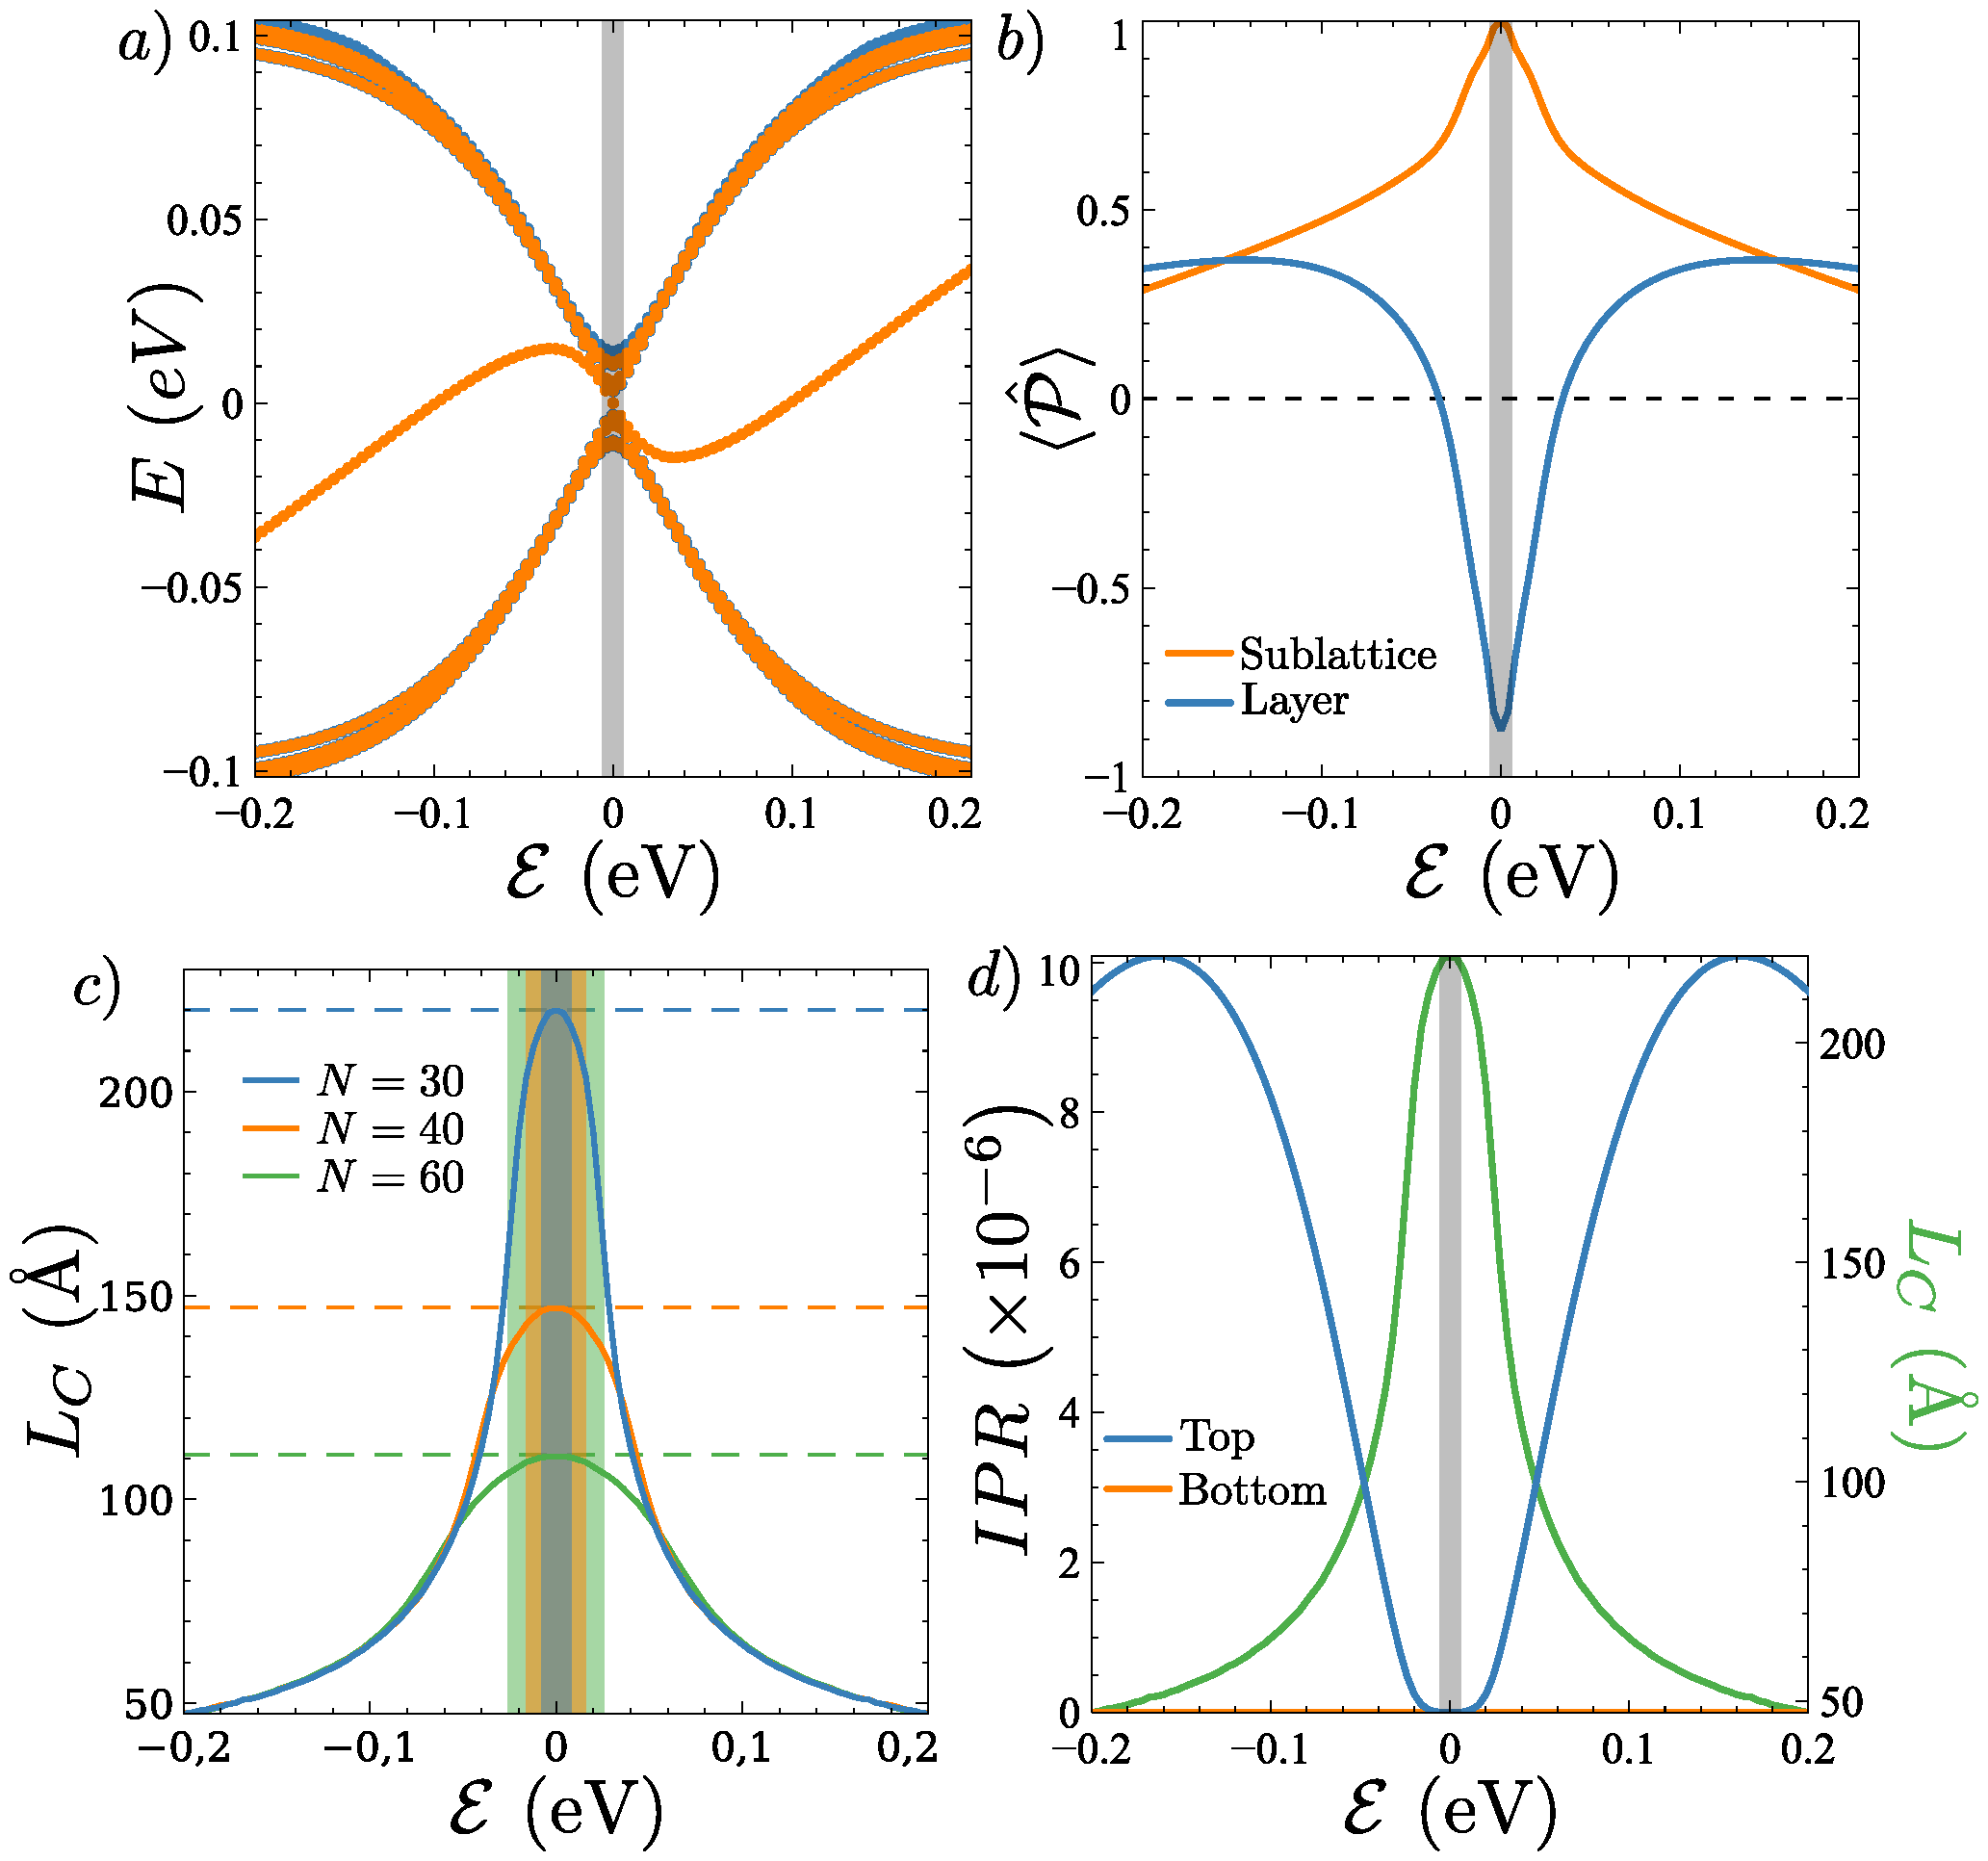
\includegraphics[width=0.7\textwidth]{artlat/fig/spectrum.pdf}
\vspace{-10pt}
\caption{$a)$ Evolution of the 9 closest eigenstates of the spectrum of an armchair island with the electric field. $b)$ Sublattice and Layer polarization as a function of the electric field. $c)$ Confinement length as defined in the main text for islands of different size. The colored areas show the regions where $|\mathcal{E}|\leqslant2\Delta_0$. The dashed lines are the length of the apothem. Notice how for $|\mathcal{E}|\to0$ the in-gap state spreads as much as it is allowed but it quickly converges for stronger electric fields. $d)$ Evolution of the IPR for the top (blue) and bottom layer (orange, $\text{IPR}_b\sim10^{-11}$ barely visible at the bottom). While the bottom \ac{ipr} is almost constant, for the top layer it changes five orders of magnitude with the electric field, showing how much the in-gap state can be confined. The confinement length was added in green for comparison}
\label{spectrum}
\end{figure}
% \FloatBarrier
%~~~~~~~~~~~~~~~~~~~~~~~~~~~~~~~~~~~~~~~~~~~~~~~~~~~~~~~~~~~%
In \fref{spectrum} we see the evolution of different properties with the electric field. Panel $a)$ shows the deformation of the spectrum of the island with the electric field. The in-gap state appears consistently in the middle of the gap but its position does not change monotonously. This behavior is understood by the interplay between the external electric field and the charge polarization induced as a respond to it.

We can build up our intuition about it by estimating the expected energy of the in-gap state. A first order perturbative calculation yields an expected energy for the in-gap state (remember \eqref{Helec}):
\begin{equation}
   E_0 (\mathcal{E}) = \mathcal{E} \bra{\Psi_0}\hat{L}\ket{\Psi_0}
\end{equation}
where $\hat{L}$ is the layer operator. In order to understand the implications of this, let us consider a vacancy in the upper layer ($\lambda_l=+1$). At $\mathcal{E}=\SI{0.0}{eV}$, the in-gap state, $\Psi_0$, is quite layer-polarized: $\bra{\Psi_0}\hat{L}\ket{\Psi_0}\sim-0.8$. It is expected that in the presence of an electric field the in-gap state would shift with a negative slope since the energy is proportional to the charge (negative for the electron) and the electric field, roughly: $E\propto q\cdot \mathcal{E}$ with the appropriate units. This initial polarization happens to oppose the electric field so for $|\mathcal{E}|\sim0$ still prevails until the electric field is overcomes the natural polarization and dominates the evolution of the in-gap state, changing the sign of the slope.

% This behavior suggests a crossover between two interactions: the electric field and the kinetic terms. Let us study the effects of the interlayer coupling in this system.

As the electric fields becomes stronger, we can see that the in-gap state looses its initial polarization, \fref{spectrum}b), reaching a stable distribution between both layers and sublattices.
The sublattice polarization behaves as expected. As the electrons are forced across the layers by the electric field they are forced to switch sublattices (notice that in $AB$-stacked bilayer the only inter-layer hoppings connect $A$ atoms of one layer to $B$ atoms in the other). As a result the sublattice polarization decreases monotonously with the electric field

The most relevant effect introduced by the electric field is the localization of the in-gap state. \fref{spectrum}c) shows the strong reduction of the confinement length, $L_c$, defined as:
\begin{equation}
  0.9 = \int_{r_0}^{L_C} \Psi_0(r) dr   %XXX arreglar!!!
\end{equation}
This non-standard definition gives an intuitive idea of how localized the in-gap state is around the vacancy, placed at $r_0$. This threshold, somewhat arbitrary, was chosen because the ratio between the area of a hexagon and its inscribed circle is around $0.9$. Here it is quick proof, for a hexagon of side $l$ and apothem $x=\sqrt{3}l/2$:
\begin{equation}
\begin{split}
   A_{\text{hex}} = 6\frac{lx}{2} = \frac{3\sqrt{3}}{2}l^2 &\qquad;\qquad
   A_{\circ} = \pi x^2 = \frac{3\pi}{4}l^2 \\
   \frac{A_\circ}{A_{\text{hex}}} = \frac{\pi}{2\sqrt{3}} &\simeq 0.906899\dots
\end{split}
\end{equation}

Other metric to estimate the localization of the in-gap state is the \acf{ipr}, defined as:
\begin{equation}
  \ket{\Psi_0} = \sum_\beta c_\alpha\ket{\phi_\alpha}\quad\quad;\quad\quad
  \text{IPR} = \sum_\alpha |c_\alpha|^4
\end{equation}
Let us keep in mind that the smaller the IPR, the more spread the state is. In the limit case in which a given state is equally spread over all the $N$ available atoms, the IPR would be $\text{IPR}=1/N$, while for a state localized in a single atom, it would be $\text{IPR}=1$.
It is interesting to see how different the \ac{ipr} for the top and bottom layers behave.
For the bottom layer, the IPR is very small ($\sim10^{-11}$) and it barely changes with the electric field. This shows an extended state no matter the applied electric field.
That is not the case for the top layer. In the top layer the $\text{IPR}\sim0$ for very small electric fields, but it increases rapidly with the electric field, showing that the state gets quickly localized.
\medskip

Both quantities give us a good idea of the physics of the system. For $\mathcal{E}=0$ the in-gap state is completely delocalized in the bottom layer, but centered around the defect in the top layer.
As the electric field is increased, the bottom layer loses spectral weight reducing the layer polarization and the in-gap state gets confined around the defect as shown both in the \ac{ipr} and the confinement length.
\smallskip

The smallest localization length is a robust result. Even for small islands it seems like the in-gap state can be reduced to $\sim\SI{50}{\angstrom}$.
\smallskip

This results gives us the scale at which we will be able to find interesting physics. If two (or more) defects are placed say $\sim\SI{100}{\angstrom}$ apart, the electric field would allow us to switch off the interactions between them by confining them.





%   \subsection{Role of the interlayer coupling}
%   Naively, one may expect the in-gap state to shift linearly with the electric field as, for instance, the conduction and valence states do. Nevertheless, the calculations show otherwise.
%   For small electric fields (we will discuss this scale later on) the in-gap state moves in opposition to the electric field, as discussed in \fref{spectrum}a).
%   %~~~~~~~~~~~~~~~~~~~~~~~~~~ FIGURE ~~~~~~~~~~~~~~~~~~~~~~~~~%
%   \begin{figure}[!ht!]
%   \centering
%   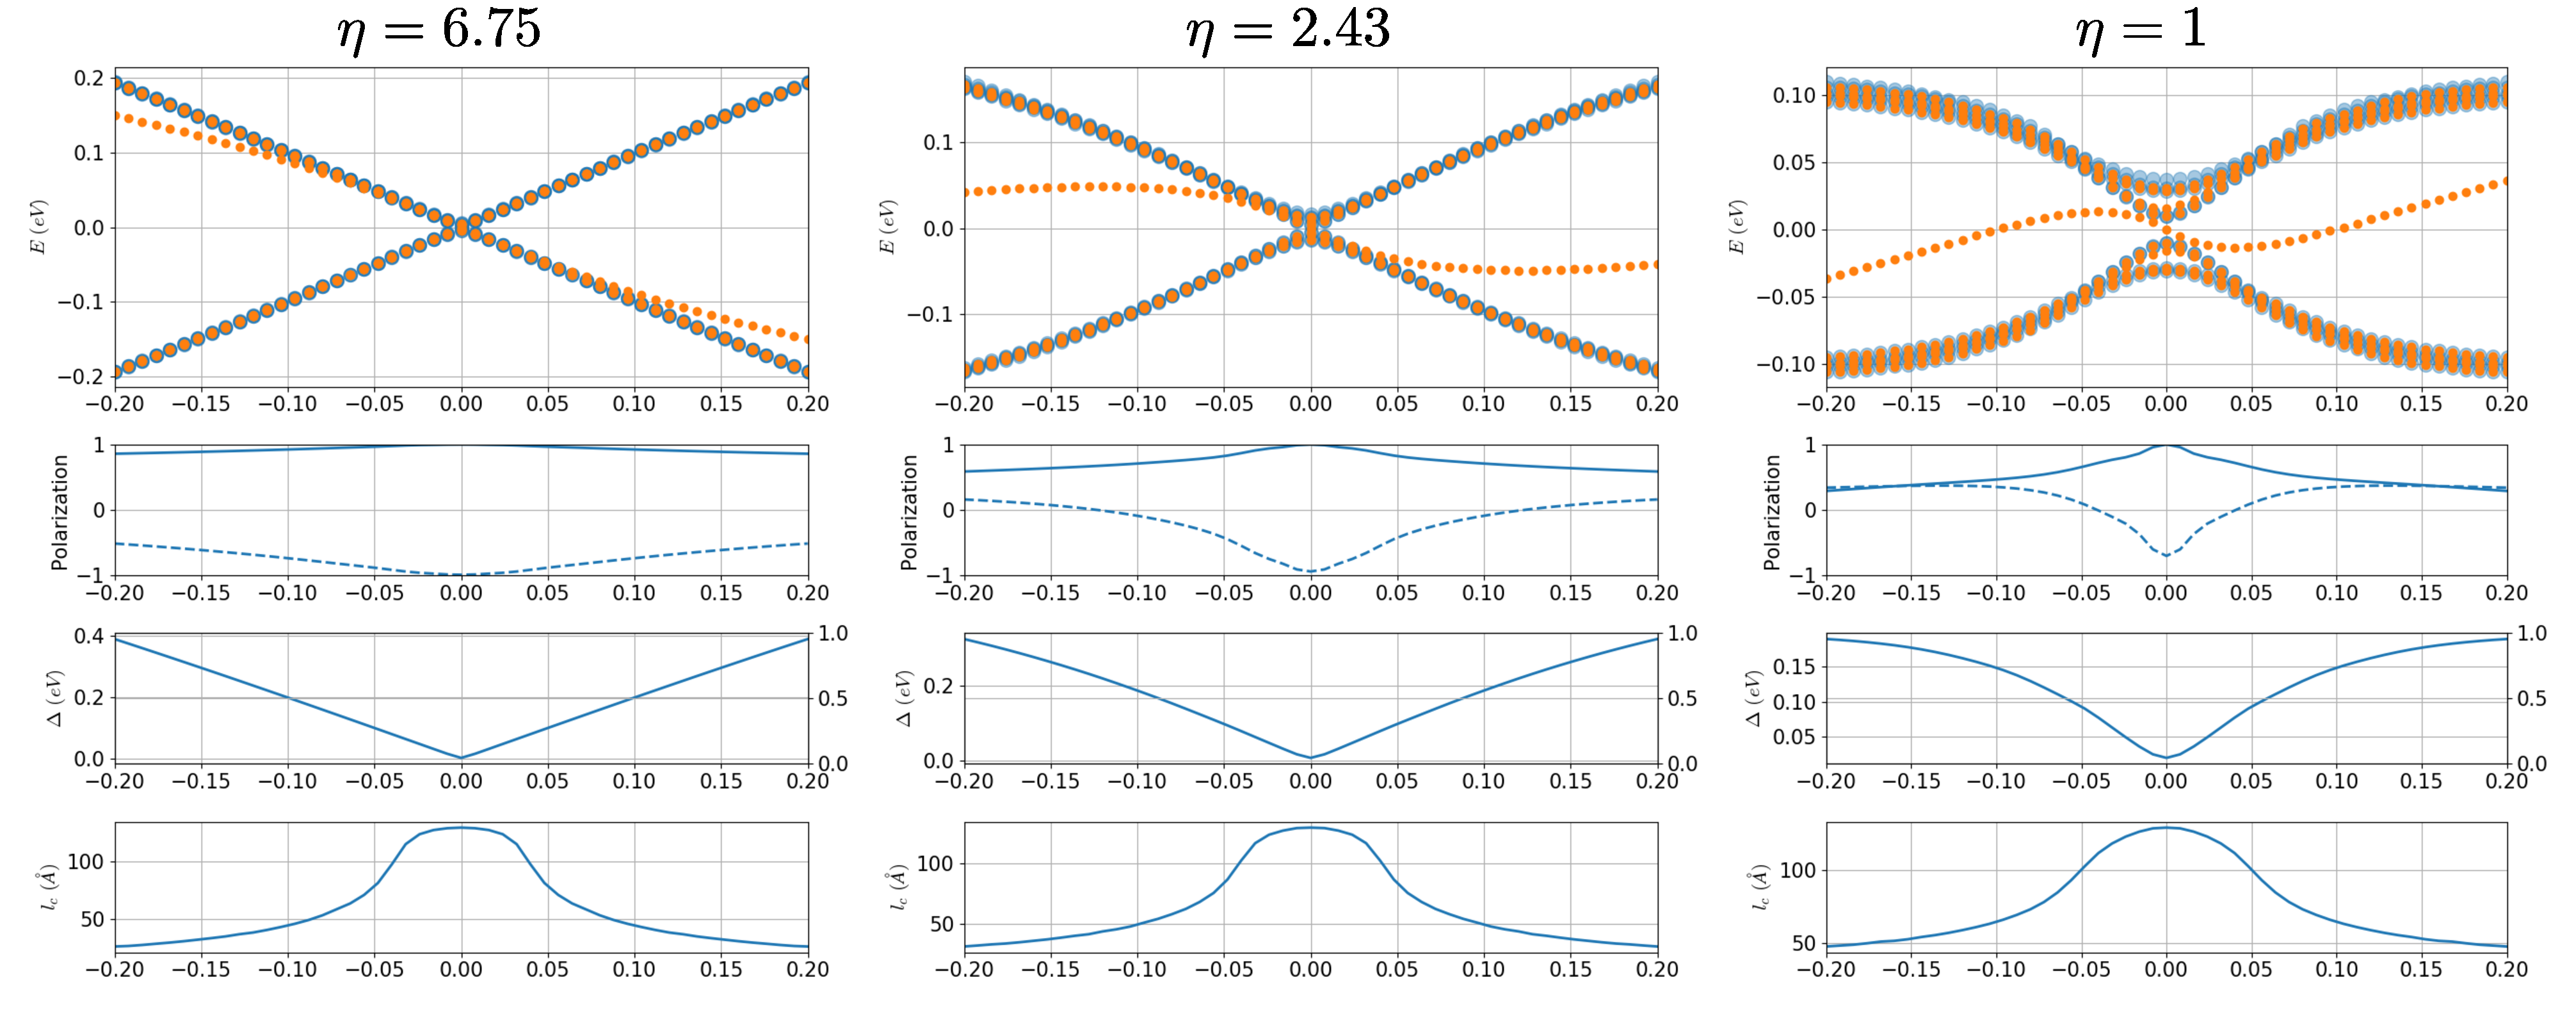
\includegraphics{artlat/fig/ingap_interlayer.pdf}
%   \vspace{-15pt}
%   \caption{Evolution of the spectrum with the interlayer coupling. The left panel shows the spectrum if we consider interlayer interactions as strong as the intralayer ones. The right panel shows the realistic value and the central panel shows an intermediate situation.}
%   \label{ingap_interlayer}
%   \end{figure}
%   % \FloatBarrier
%   %~~~~~~~~~~~~~~~~~~~~~~~~~~~~~~~~~~~~~~~~~~~~~~~~~~~~~~~~~~~%
%   For large electric fields the in-gap state does move linearly with the electric field, yet, the rate at what it does depends strongly on the interlayer coupling, as shown in \fref{ingap_interlayer}.
%   We will consider the Hamiltonian of the system to be two graphene hamiltonians coupled by an interlayer interaction:
%   \begin{equation}
%     H = H_{\text{L}_1} + \eta H_{\text{inter}} + H_{\text{L}_2}
%   \end{equation}
%   The intralayer $\pi$-hoppings are $t=\SI{-2.7}{\eV}$ while the interlayer hoppings (which are $\sigma$-hoppings, due to the symmetry of the orbitals) are roughly $t_{\text{inter}}=\SI{0.4}{\eV}$. $\eta$ is an artificial adimensional parameter that will allow us to tune the interlayer coupling to study the behavior of the system. In this fashion, $\eta=1$ corresponds to normal, realistic GBL, while $\eta=0$ describes two decoupled graphene layers and, in particular, $\eta=6.75$ corresponds to having an \emph{inter}layer coupling as strong as the \emph{intra}layer one.\\
%   
%   In order to understand the role of the interlayer coupling in the in-gap state, it is useful to plot the dependence of the layer polarization with the parameter $\eta$. We consider this parameter to range from 0.5 (slightly decouple) to 6.75 (strongly coupled so inter and intralayer hopping is the same).
%   %~~~~~~~~~~~~~~~~~~~~~~~~~~ FIGURE ~~~~~~~~~~~~~~~~~~~~~~~~~%
%   \begin{figure}[!ht!]
%   \centering
%   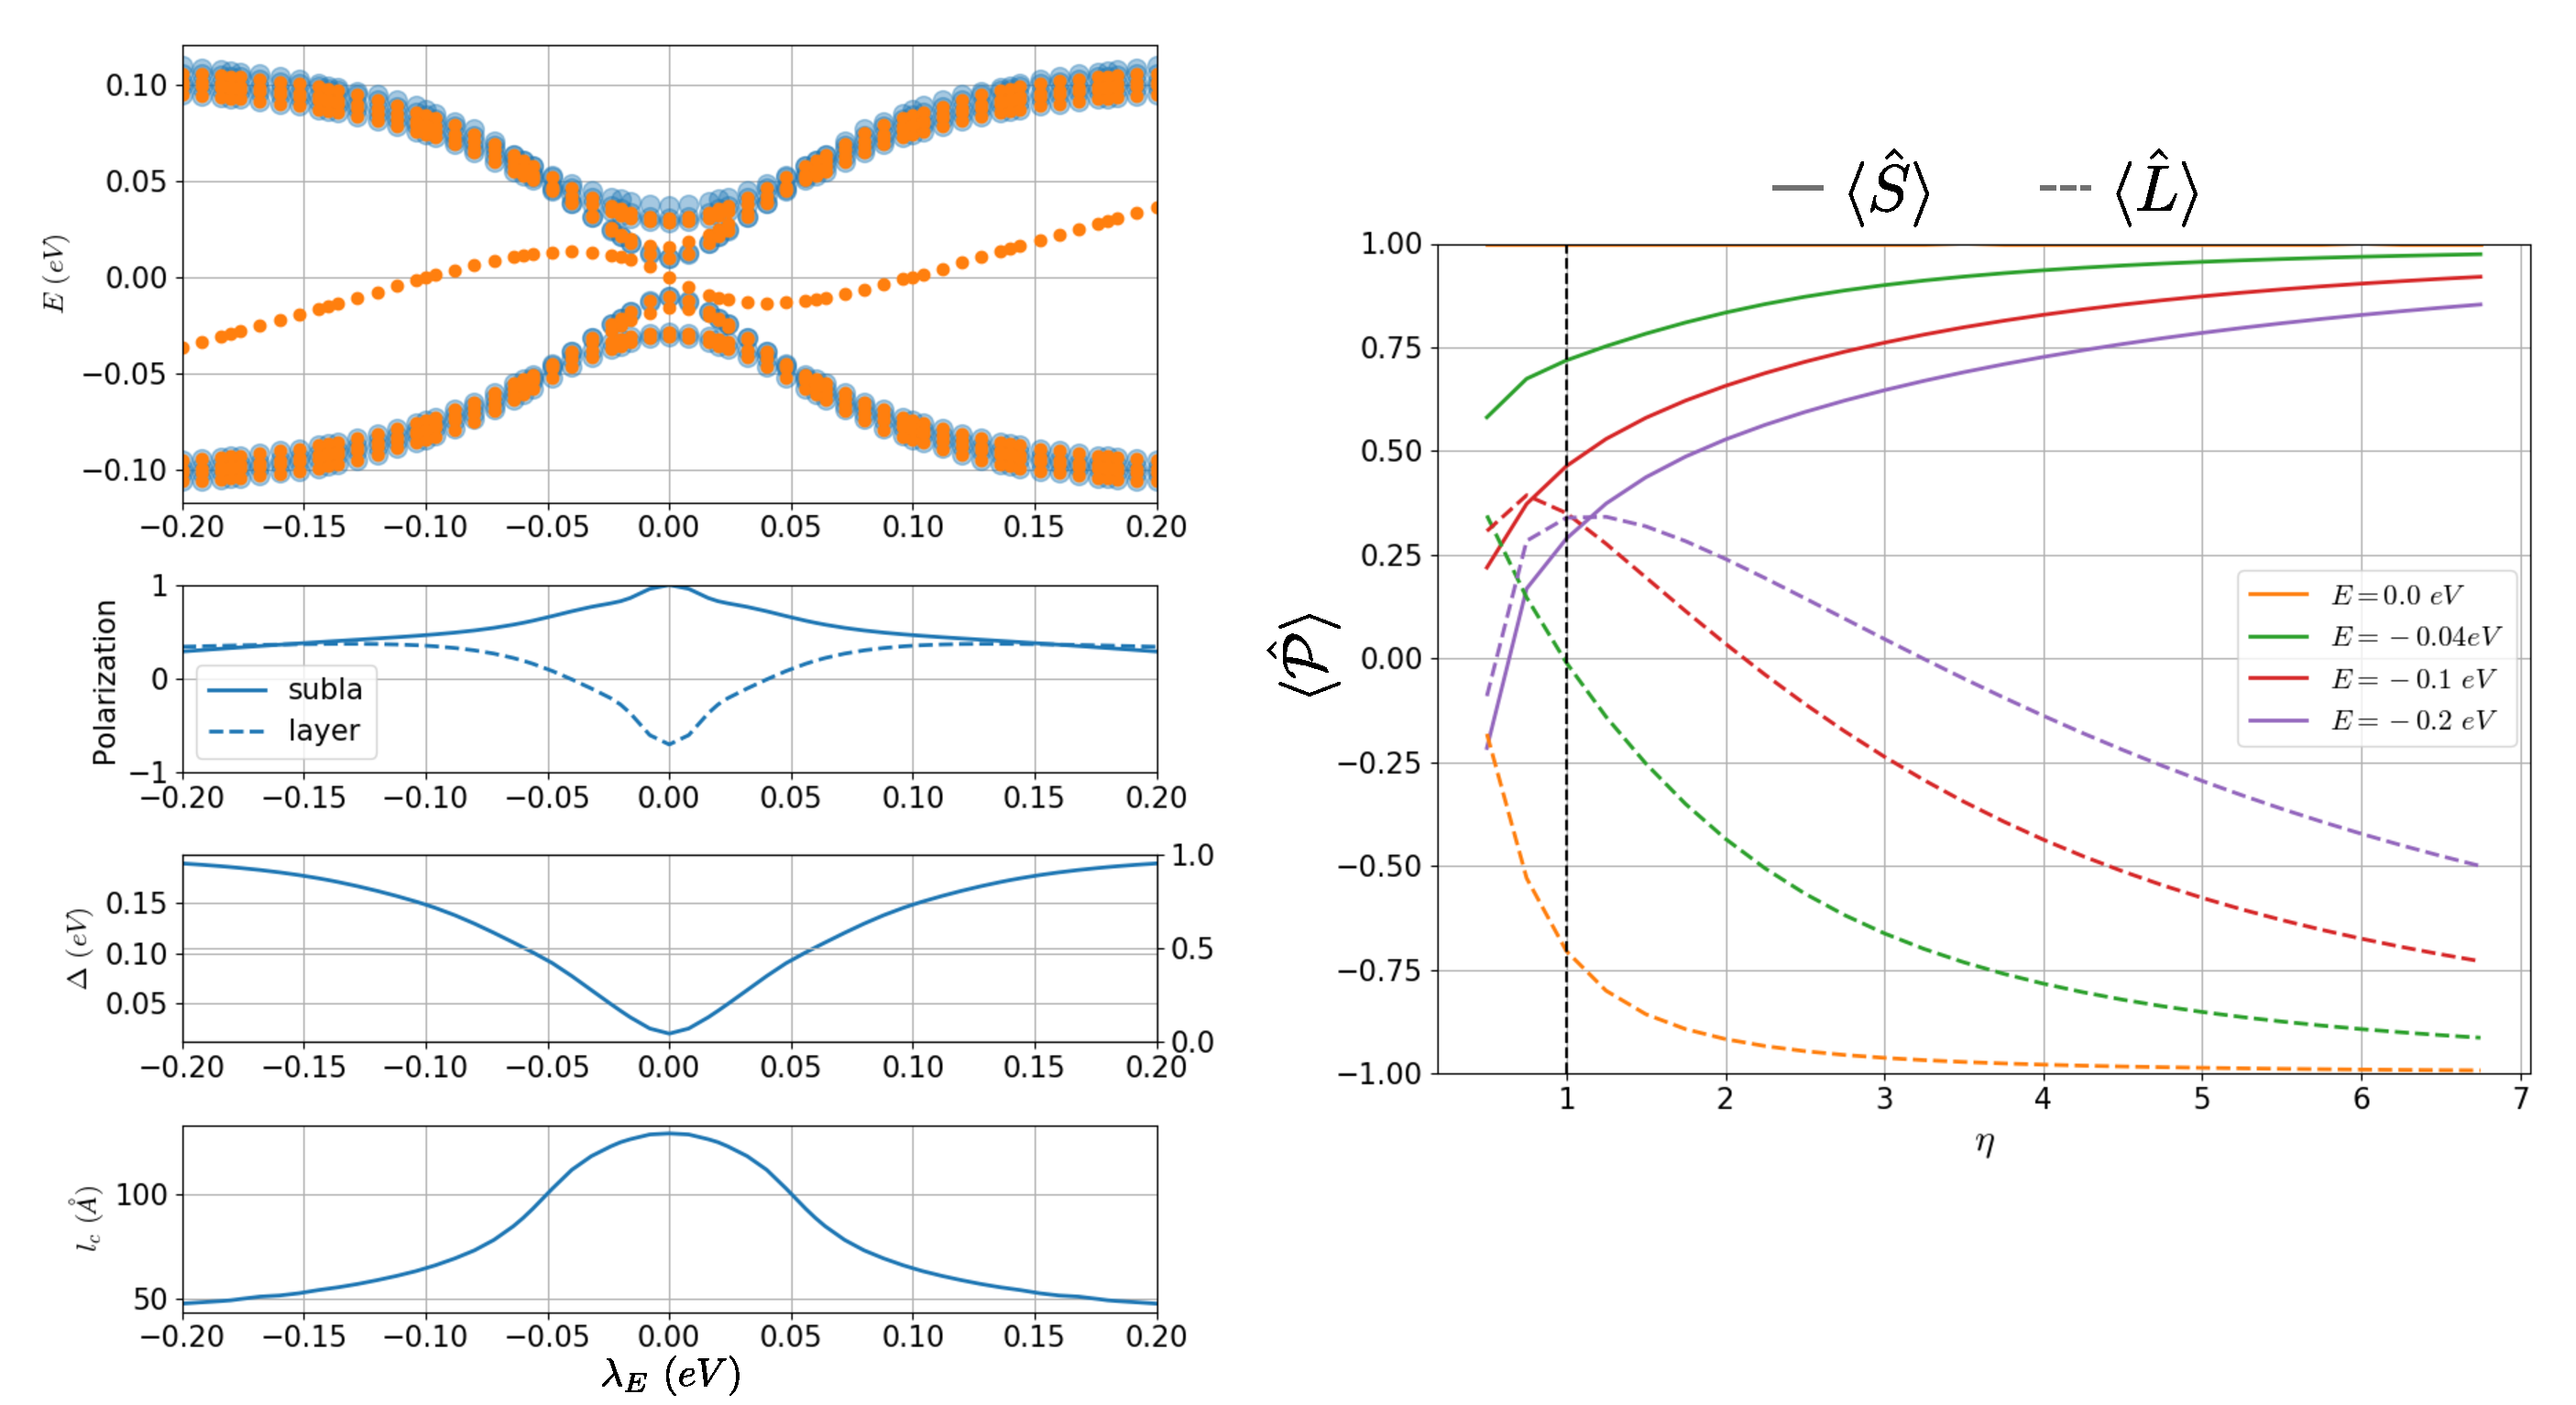
\includegraphics[width=\textwidth]{artlat/fig/polarization.pdf}
%   \vspace{-15pt}
%   \caption{$a)$ Evolution of different properties with the electric field. First panel shows the evolution of the spectrum, the second one shows the sublattice and layer polarizations, the third one plots the gap of the system and the forth one shows the confinement length. $b)$ Evolution of the layer (dashed lines) and sublattice polarization (solid lines) with the interlayer coupling. Notice that at zero electric field, $V=\SI{0.0}{\eV}$, the sublattice polarization remains constant at $\langle\hat{S}\rangle=1$, as expected from the Lieb's theorem.}
%   \label{pol}
%   \end{figure}
%   \FloatBarrier
%   %~~~~~~~~~~~~~~~~~~~~~~~~~~~~~~~~~~~~~~~~~~~~~~~~~~~~~~~~~~~%
%   We can see that the electric field overcomes the interlayer contribution when the system reaches charge neutrality $\langle\hat{L}\rangle=0$.
%   
%   We can try to understand this step by step. When a H adatom is introduced (aka, a vacancy), one electron is localized in the vicinity of the defect. %The three closest atoms bear most of the spectral weight of this state, and the rest spreads all over the island but only in one sublattice.
%   For an adatom chemisorbed on top of a C atom belonging to the sublattice -1 in the top layer (namely 1), the sublattice and layer polarization are:
%   \begin{equation*}
%     \langle\hat{S}\rangle = 1 \quad;\quad
%     \langle\hat{L}\rangle = -0.7
%   \end{equation*}
%   
%   This means that the in-gap state is completely sublattice polarized (as Lieb's theorem predicts) but it is only $\sim70\%$ layer polarized, meaning that the localized electron lives mostly \textbf{in the layer that does not contain the vacancy}.
%   
%   If we artificially increase the value of the interlayer coupling we can that the layer polarization consistently drops to lower values, showing that the in-gap state prefers to spread in the layer that does not contain the vacancy. Analogously, the evolution of the sublattice polarization also shows that the in-gap state gets more and more sublattice-polarized.
%   
%   This behavior might be understood keeping in mind the behavior of a single vacancy in graphene. It is known that for a vacancy in graphene, the in-gap state is mostly concentrated in the three closest atoms. In graphene bilayer it happens that these three closest atoms are connected to the other graphene layer, so the stronger the interlayer coupling, the easier will be for the in-gap state to spread to the other layer.

% XXX
% What I do not understand is that the 3 atoms closest to the vacancy (containing most of the state at $\eta=0$) are connected to atoms of the opposite sublattice in the other layer, yet, the sublattice polarization seems to keep its expected flavor even when the interlayer coupling is heavily increased.















% \newpage
% Since we are studying an island with a single vacancy, the energy levels are a discrete set of energies. In figure~\ref{1vac_spec} (c) the difference in the spectrum due to the introduction of a vacancy at $\lambda_E=0$ is shown. When a vacancy is introduced, an in-gap state appears at $E=0$ and some \emph{(quasi-)}degeneracies are broken.
%
% The effect of the electric field in the spectrum is shown in figure~\ref{1vac_spec} $a)$ and $b)$. Its main effect is to open a gap, linearly dependent with the electric field.
%
% The shift in the energy at which the in-gap state appears is linear for low electric field, but it remains in-gap for all the regime of electric fields studied. In fig~\ref{1vac_spec} $a$-$c)$ only the eight eigenvalues closest to $E=0$ are plotted. Nevertheless, since the spacing between levels is much smaller than the gap open by the electric field, they appear grouped in two sets of almost-degenerate energies, one at $E>0$ and the other at $E<0$.\\
%
% %~~~~~~~~~~~~~~~~~~~~~~~~~~ FIGURE ~~~~~~~~~~~~~~~~~~~~~~~~~%
% \begin{figure}[!ht!]
% \centering
% 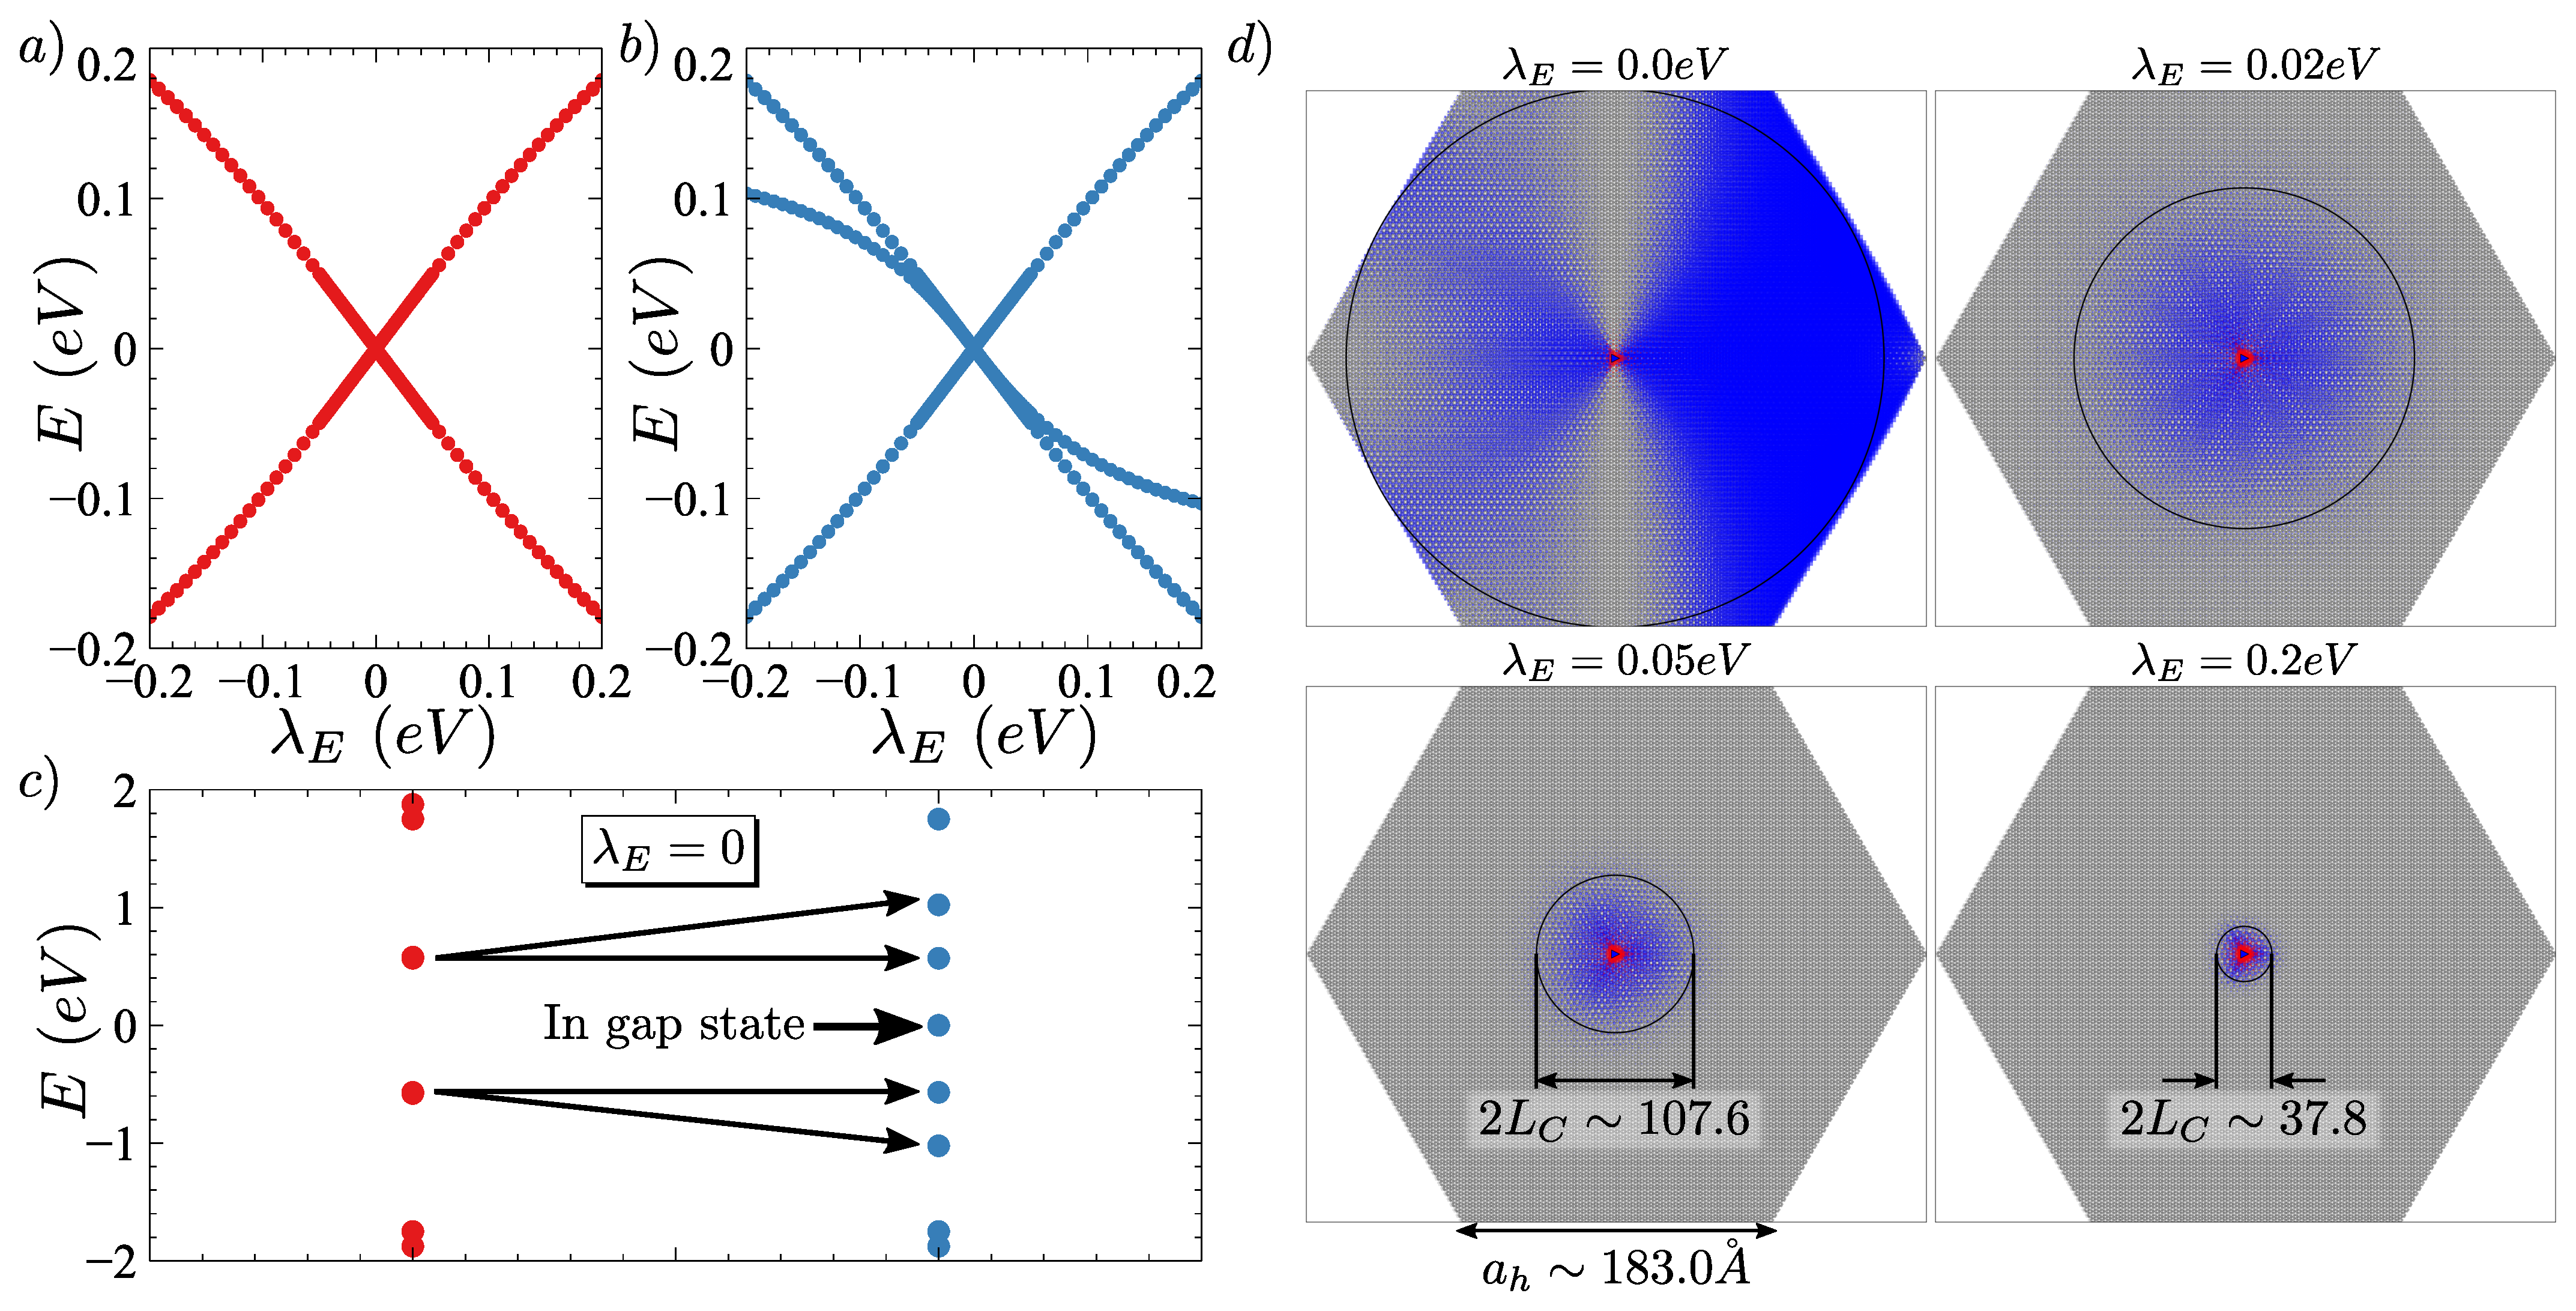
\includegraphics[width=\textwidth]{single_vac_spectrum.pdf}
% \vspace{-15pt}
% \caption{$a)$ and $b)$ show the pristine and defected spectrum respectively as a function of different applied electric fields. Notice the opening of a gap linear with the electric field (in both the pristine and defected cases) and the appearance of an extra state inside the gap. $c)$ Pristine (red) and defected (blue) spectrum for the case of no electric field $\lambda_E=0$. Panel $d)$ shows four snapshots of an island ($N_C=91812$ atoms) at different values of the electric field. The black circle in panel $d)$ shows the confinement length $L_C$ defined in the text.}
% \label{1vac_spec}
% \end{figure}
% \FloatBarrier
% %~~~~~~~~~~~~~~~~~~~~~~~~~~~~~~~~~~~~~~~~~~~~~~~~~~~~~~~~~~~%
%
% In Fig~\ref{1vac_spec} $d)$ we show four snapshots of the spatial distribution of the in-gap state. The actual lattice of the island is shown as black dots (probably indistinguishable because of the size of the image).
% On top of each atomic position the weight of the wave function ($|c_\beta|^2$ using the notation of eq.~\eqref{general}) is plotted in blue/red for the lower/upper layer.
% On top of all this, the site of the vacancy is marked with a blue triangle.
% As a visual guide the confinement length is plotted as a black circle with diameter $2L_C$.\\
%
% At $\lambda_E=0$ the system is bipartite, so according to the Lieb's theorem, after the removal of one site, a sublattice-polarized state should appear at $E=0$. This is exactly what happens as shown in Fig.~\ref{1vac_spec}.
%
% When we study the real-space distribution of the in-gap state we find that in the absence of electric field ($\lambda_E=0$) the state is spread all over the island, Fig.~\ref{1vac_spec} $d)$, no matter the size of the island (see Fig.~\ref{IPR_lc} $a)$ bellow). Notice that the effect of the border is not negligible in this regime and, in fact, is the responsible of the breaking of the expected $C_3$ symmetry of the state (at long distances, close to the vacancy the $C_3$ symmetry is almost preserved).
%
%
% Another important aspect is that the distribution of this wave function is such that in the upper layer (the one containing the vacancy) the wave function is quite confined around the vacancy (3-6 closest atoms) and it barely changes with the electric field, whereas in the lower layer the spreading of the wave function varies from the whole space available, to a few angstroms.
%
%
% To study quantitatively the properties of the in-gap state $\psi_0$ we define four quantities that will be useful later on.
% \begin{itemize}
%   \item \emph{Confinement length}, $L_C$, defined, hand-wavingly, as the distance at which more than $90\%$ of the state is located
%   \begin{equation}
%     0.9 = \int_{0}^{L_C} \psi_0(r) dr   %XXX arreglar!!!
%     \label{loclen}
%   \end{equation}
%   This confinement length can be used as a measurement of the spreading of the in-gap state $\psi_0$.
%   \begin{equation}
%     L'_C = \bra{\psi_0} |R-r_0|^2\ket{\psi_0}
%   \end{equation}
%   \item \emph{Inverse participation ratio} (IPR), $\eta$. Using the notation of equation~\eqref{general}, the IPR can be defined as:
%   \begin{equation}
%     \ket{\psi_0} = \sum_\beta c_\beta\ket{\phi_\beta}\quad\quad;\quad\quad
%     \text{IPR} = \eta = \sum_i |c_\beta|^4
%   \end{equation}
%   \item \emph{Sublattice} and \emph{Layer polarization}, defined as the expected value of the in-gap state.
%   \begin{equation}
%     SP = \bra{\psi_0}\widehat{\mathcal{S}}\ket{\psi_0}
%     \quad\quad;\quad\quad
%     SL = \bra{\psi_0}\widehat{\mathcal{L}}\ket{\psi_0}
%   \end{equation}
%   where the operators $\widehat{\mathcal{S}}$ and $\widehat{\mathcal{L}}$ measure the component of a given state in a given sublattice and layer respectively. Both $SP$ and $SL$ have to be, by definition, in the closed interval $\left[-1,1\right]$.
% \end{itemize}
%
% In figure~\ref{IPR_lc} we study the dependence of these four properties, for different sizes of the island, as a function of the electric field.
% %~~~~~~~~~~~~~~~~~~~~~~~~~~ FIGURE ~~~~~~~~~~~~~~~~~~~~~~~~~%
% \begin{figure}[!ht]
% \centering
% 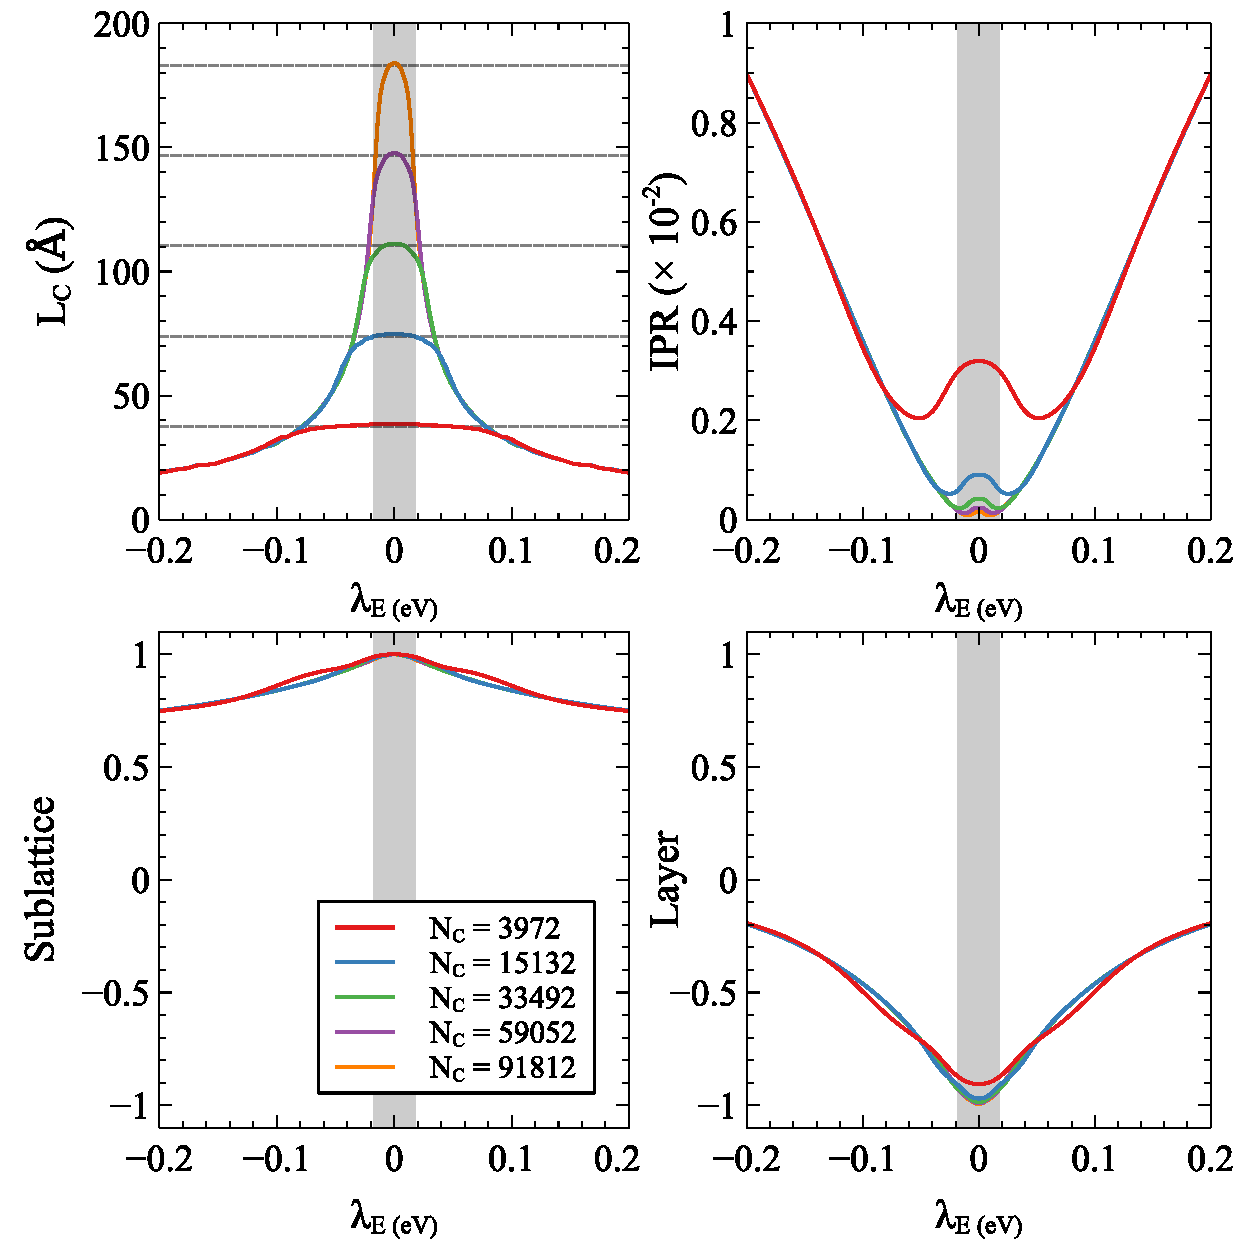
\includegraphics[width=0.6\textwidth]{single_vac_properties.pdf}
% \vspace{-5pt}
% \caption{$a)$ Dependence of the localization length $L_c$ with the electric field for different sizes of the island. The dashed lines corresponds to the size of the each corresponding island. $b)$ IPR, $\eta$, dependence with the electric field for different sizes of the island. $c)$ and $d)$ show the degree of sublattice and layer polarization for different sizes of the island as a function the electric field. The values $\pm1$ refer to $A/B$ sublattice or up/down layer respectively.}
% \label{IPR_lc}
% \end{figure}
% \FloatBarrier
% %~~~~~~~~~~~~~~~~~~~~~~~~~~~~~~~~~~~~~~~~~~~~~~~~~~~~~~~~~~~%
%
% It can be seen in Fig.~\ref{IPR_lc} $a)$ that as we approach the limit $\lambda_E\rightarrow0$ the confinement length collapses to the size of the island, shown as a dashed line for each size studied. This plateau is just the effect of having an in-gap state spread all over the island.
%
% The shadowed region in all the panels shows the range of $\lambda_E$ in which the border effects can be relevant for the biggest island studied ($N_C=91812$). It is estimated as the $\lambda_E$ at which the results differ from those of the previous island. Of course it is only a rough estimation and it should be considered only as a guide to the eye when reading the results.
%
% In panel $b)$ the IPR is shown. Except for small islands the evolution of the IPR, as that of the $L_C$, is the same regardless of the size of the island. The increasing of the IPR with the electric field is another sign of the increasing localization of the in-gap state around the vacancie.\\
%
% The sublattice and layer polarization are shown in panels~\ref{IPR_lc} $c)$ and $d)$. As it can be seen at $\lambda_E=0$ the state is completely sublattice-polarized, in accordance with the Lieb's theorem, and almost layer-polarized, this almost is more easly visible in the small red component present in Fig.~\ref{1vac_spec} $d)$.
%
% As the electric field increases the bipartite character of the system is lost, in agreement with the shift of the energy of the in-gap state (no longer at $E=0$). Since the system is no longer bipartite, the sublattice polarized character of the in-gap state is no longer assured, and as shown in panel $c)$ it, in fact, decreases.
%
% The decreasing of the layer polarization is easily understood by looking at Fig.~\ref{1vac_spec} $d)$. For small $\lambda_E$ the in-gap state is mostly spread over the lower layer, while for large $\lambda_E$ the in-gap state occupies roughly the same area in both layers resulting in a $\bra{\psi_0}\widehat{\mathcal{L}}\ket{\psi_0} \rightarrow 0$
%
%
%
%
% % When a single $p_z$ site is removed from graphene, an electron is confined in the surroundings of the vacancy with energy $E=0$. While it is true that such a state is mainly localized in the 3 closest neighbors, the rest of the state is diluted in all the other available sites. \red{[non-renormalizable?]}
% %
% % Interestingly, when a gap is open, the state becomes normalizable and a confinement length can be defined. In particular, the confinement length is controlled by the size of the gap.
% %
% % Graphene bilayer shows a tuneable band gap when an external electric field is applied\cite{}. This manipulation of the gap provides an excellent tool to control the confinement of any in-gap state.
% %
% % We will use an island of graphene bilayer with 91812 atoms. The removal of the hollow site closest to the center of the island results in an in-gap state as shown in Fig~\ref{single_vac}.
% %
% % %~~~~~~~~~~~~~~~~~~~~~~~~~~ FIGURE ~~~~~~~~~~~~~~~~~~~~~~~~~%
% % \begin{figure}[h!]
% % \centering
% %   \includegraphics[width=0.7\textwidth]{single_vacancy.pdf}
% % \vspace{-5pt}
% % \caption{Effect of an external electric field in the ingap state of a graphene bilayer with a single vacancy \red{include bands}}
% % \label{single_vac}
% % \end{figure}
% % \FloatBarrier
% % %~~~~~~~~~~~~~~~~~~~~~~~~~~~~~~~~~~~~~~~~~~~~~~~~~~~~~~~~~~~%

%%~~~~~~~~~~~~~~~~~~~~~~~~~~ FIGURE ~~~~~~~~~~~~~~~~~~~~~~~~~%
%\begin{figure}[h!]
%\centering
%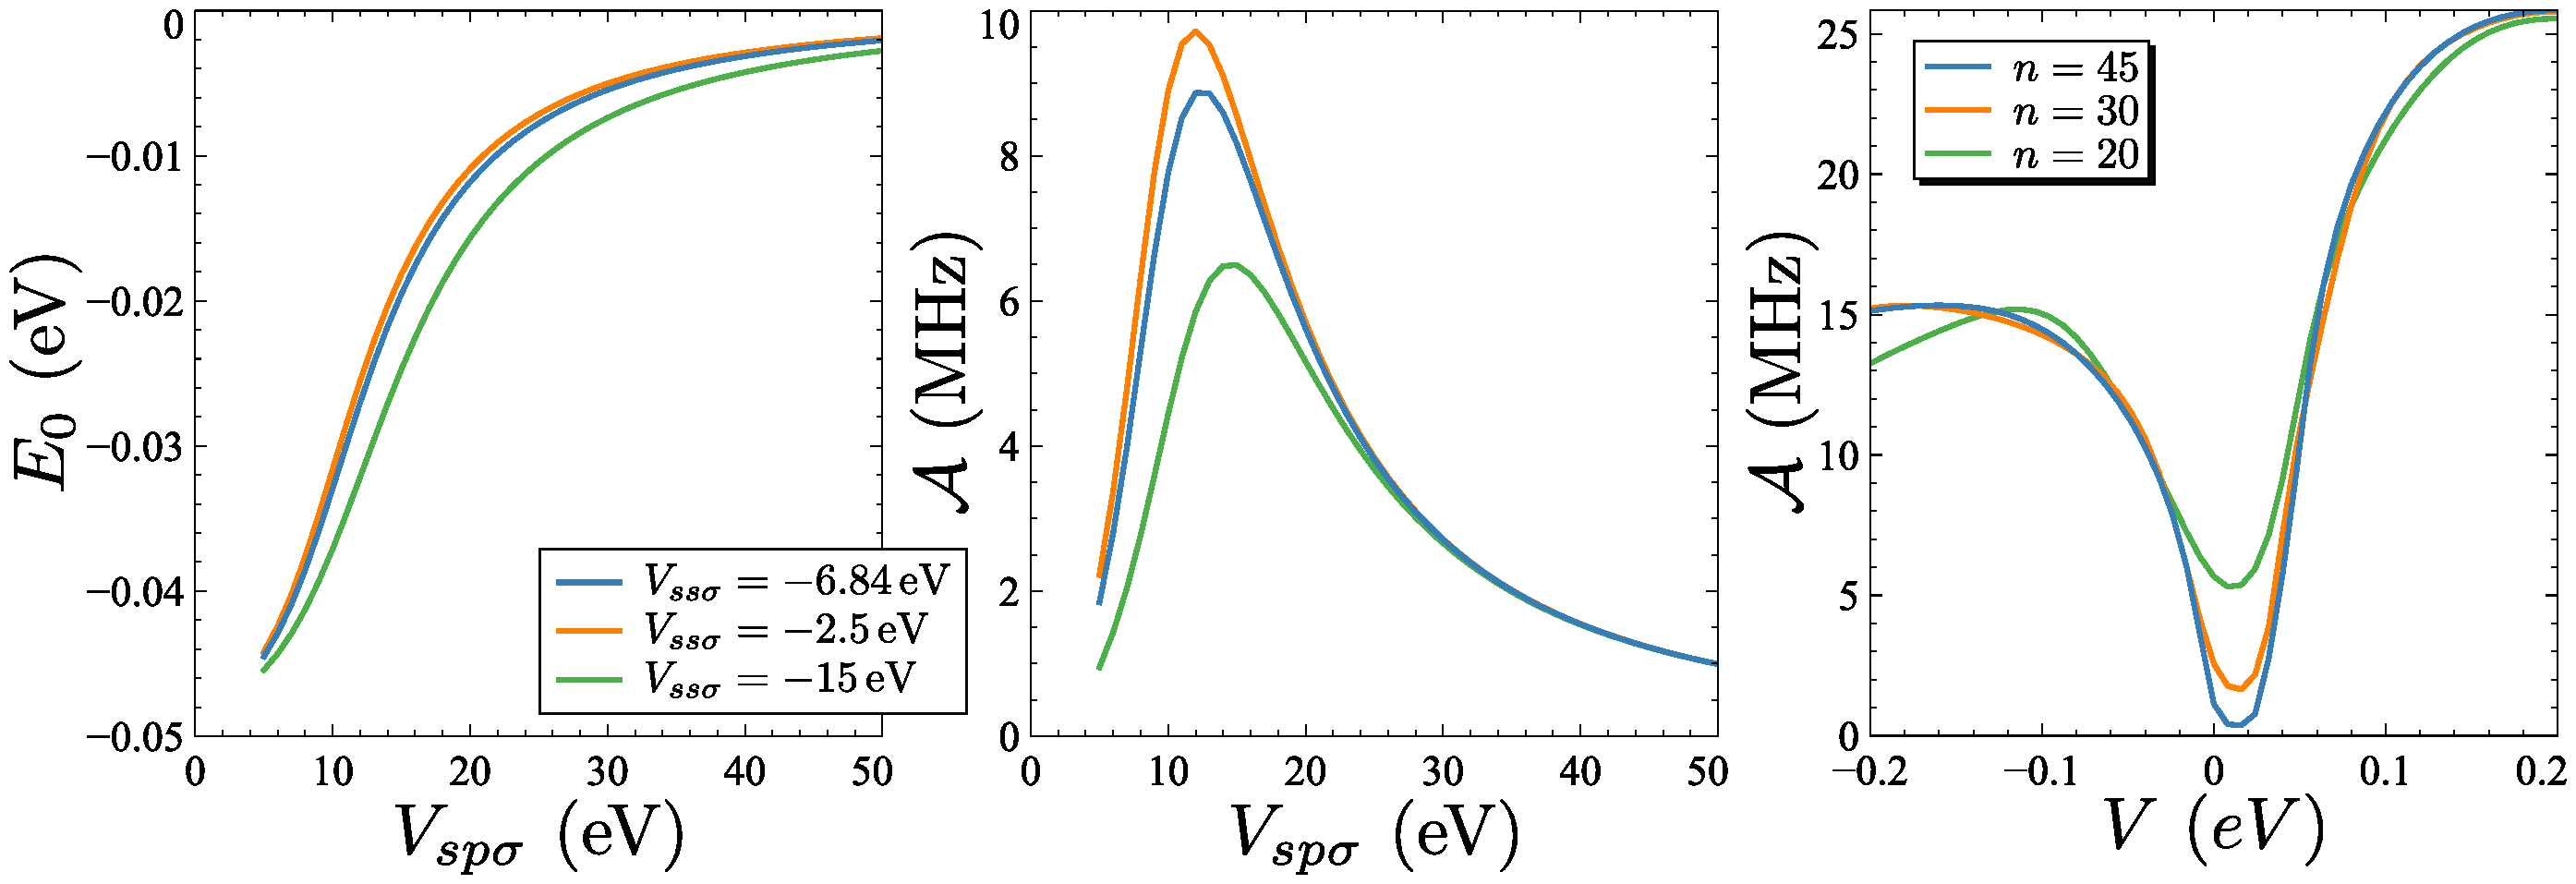
\includegraphics{artlat/fig/hyperfine.pdf}
%\vspace{-20pt}
%\caption{Change in the hyperfine coupling with the electric field.}
%\label{latt_hyper}
%\end{figure}
%\FloatBarrier
%%~~~~~~~~~~~~~~~~~~~~~~~~~~~~~~~~~~~~~~~~~~~~~~~~~~~~~~~~~~~%
